%\documentclass[a4paper,11pt,twocolumn]{article}
\documentclass{scrreprt}
\usepackage{url}
\usepackage{listings}
\usepackage{appendix}
\usepackage{amssymb}
\usepackage{pifont}
\usepackage{makeidx}
\usepackage{fancybox}
\makeindex

\usepackage[usenames,dvipsnames]{color}
\usepackage[T1]{fontenc}
\usepackage{wrapfig}
\usepackage[pdftex]{graphicx}
\usepackage{setspace}

\usepackage[Sonny]{fncychap}
%\usepackage[Bjornstrup]{fncychap}

\usepackage[automark]{scrpage2}

\usepackage{hyperref}
\usepackage{xcolor}

\hypersetup{
    colorlinks, linkcolor={BlueViolet},
    citecolor={BrickRed}, urlcolor={NavyBlue}
}


\definecolor{lightgray}{rgb}{.9,.9,.9}
\definecolor{darkgray}{rgb}{.4,.4,.4}
\definecolor{purple}{rgb}{0.65, 0.12, 0.82}

\lstdefinelanguage{JavaScript}{
  keywords={typeof, new, true, false, catch, function, return, null, catch, switch, var, if, in, while, do, else, case, break},
  keywordstyle=\color{blue}\bfseries,
  ndkeywords={class, export, boolean, throw, implements, import, this},
  ndkeywordstyle=\color{darkgray}\bfseries,
  identifierstyle=\color{black},
  sensitive=false,
  comment=[l]{//},
  morecomment=[s]{/*}{*/},
  commentstyle=\color{purple}\ttfamily,
  stringstyle=\color{red}\ttfamily,
  morestring=[b]',
  morestring=[b]"
}


\usepackage{colortbl}

\definecolor{AliceBlue}{rgb}{0.94,0.97,1.00}
\definecolor{AntiqueWhite1}{rgb}{1.00,0.94,0.86}
\definecolor{AntiqueWhite2}{rgb}{0.93,0.87,0.80}
\definecolor{AntiqueWhite3}{rgb}{0.80,0.75,0.69}
\definecolor{AntiqueWhite4}{rgb}{0.55,0.51,0.47}
\definecolor{AntiqueWhite}{rgb}{0.98,0.92,0.84}
\definecolor{BlanchedAlmond}{rgb}{1.00,0.92,0.80}
\definecolor{BlueViolet}{rgb}{0.54,0.17,0.89}
\definecolor{CadetBlue1}{rgb}{0.60,0.96,1.00}
\definecolor{CadetBlue2}{rgb}{0.56,0.90,0.93}
\definecolor{CadetBlue3}{rgb}{0.48,0.77,0.80}
\definecolor{CadetBlue4}{rgb}{0.33,0.53,0.55}
\definecolor{CadetBlue}{rgb}{0.37,0.62,0.63}
\definecolor{CornflowerBlue}{rgb}{0.39,0.58,0.93}
\definecolor{DarkBlue}{rgb}{0.00,0.00,0.55}
\definecolor{DarkCyan}{rgb}{0.00,0.55,0.55}
\definecolor{DarkGoldenrod1}{rgb}{1.00,0.73,0.06}
\definecolor{DarkGoldenrod2}{rgb}{0.93,0.68,0.05}
\definecolor{DarkGoldenrod3}{rgb}{0.80,0.58,0.05}
\definecolor{DarkGoldenrod4}{rgb}{0.55,0.40,0.03}
\definecolor{DarkGoldenrod}{rgb}{0.72,0.53,0.04}
\definecolor{DarkGray}{rgb}{0.66,0.66,0.66}
\definecolor{DarkGreen}{rgb}{0.00,0.39,0.00}
\definecolor{DarkGrey}{rgb}{0.66,0.66,0.66}
\definecolor{DarkKhaki}{rgb}{0.74,0.72,0.42}
\definecolor{DarkMagenta}{rgb}{0.55,0.00,0.55}
\definecolor{DarkOliveGreen1}{rgb}{0.79,1.00,0.44}
\definecolor{DarkOliveGreen2}{rgb}{0.74,0.93,0.41}
\definecolor{DarkOliveGreen3}{rgb}{0.64,0.80,0.35}
\definecolor{DarkOliveGreen4}{rgb}{0.43,0.55,0.24}
\definecolor{DarkOliveGreen}{rgb}{0.33,0.42,0.18}
\definecolor{DarkOrange1}{rgb}{1.00,0.50,0.00}
\definecolor{DarkOrange2}{rgb}{0.93,0.46,0.00}
\definecolor{DarkOrange3}{rgb}{0.80,0.40,0.00}
\definecolor{DarkOrange4}{rgb}{0.55,0.27,0.00}
\definecolor{DarkOrange}{rgb}{1.00,0.55,0.00}
\definecolor{DarkOrchid1}{rgb}{0.75,0.24,1.00}
\definecolor{DarkOrchid2}{rgb}{0.70,0.23,0.93}
\definecolor{DarkOrchid3}{rgb}{0.60,0.20,0.80}
\definecolor{DarkOrchid4}{rgb}{0.41,0.13,0.55}
\definecolor{DarkOrchid}{rgb}{0.60,0.20,0.80}
\definecolor{DarkRed}{rgb}{0.55,0.00,0.00}
\definecolor{DarkSalmon}{rgb}{0.91,0.59,0.48}
\definecolor{DarkSeaGreen1}{rgb}{0.76,1.00,0.76}
\definecolor{DarkSeaGreen2}{rgb}{0.71,0.93,0.71}
\definecolor{DarkSeaGreen3}{rgb}{0.61,0.80,0.61}
\definecolor{DarkSeaGreen4}{rgb}{0.41,0.55,0.41}
\definecolor{DarkSeaGreen}{rgb}{0.56,0.74,0.56}
\definecolor{DarkSlateBlue}{rgb}{0.28,0.24,0.55}
\definecolor{DarkSlateGray1}{rgb}{0.59,1.00,1.00}
\definecolor{DarkSlateGray2}{rgb}{0.55,0.93,0.93}
\definecolor{DarkSlateGray3}{rgb}{0.47,0.80,0.80}
\definecolor{DarkSlateGray4}{rgb}{0.32,0.55,0.55}
\definecolor{DarkSlateGray}{rgb}{0.18,0.31,0.31}
\definecolor{DarkSlateGrey}{rgb}{0.18,0.31,0.31}
\definecolor{DarkTurquoise}{rgb}{0.00,0.81,0.82}
\definecolor{DarkViolet}{rgb}{0.58,0.00,0.83}
\definecolor{DeepPink1}{rgb}{1.00,0.08,0.58}
\definecolor{DeepPink2}{rgb}{0.93,0.07,0.54}
\definecolor{DeepPink3}{rgb}{0.80,0.06,0.46}
\definecolor{DeepPink4}{rgb}{0.55,0.04,0.31}
\definecolor{DeepPink}{rgb}{1.00,0.08,0.58}
\definecolor{DeepSkyBlue1}{rgb}{0.00,0.75,1.00}
\definecolor{DeepSkyBlue2}{rgb}{0.00,0.70,0.93}
\definecolor{DeepSkyBlue3}{rgb}{0.00,0.60,0.80}
\definecolor{DeepSkyBlue4}{rgb}{0.00,0.41,0.55}
\definecolor{DeepSkyBlue}{rgb}{0.00,0.75,1.00}
\definecolor{DimGray}{rgb}{0.41,0.41,0.41}
\definecolor{DimGrey}{rgb}{0.41,0.41,0.41}
\definecolor{DodgerBlue1}{rgb}{0.12,0.56,1.00}
\definecolor{DodgerBlue2}{rgb}{0.11,0.53,0.93}
\definecolor{DodgerBlue3}{rgb}{0.09,0.45,0.80}
\definecolor{DodgerBlue4}{rgb}{0.06,0.31,0.55}
\definecolor{DodgerBlue}{rgb}{0.12,0.56,1.00}
\definecolor{FloralWhite}{rgb}{1.00,0.98,0.94}
\definecolor{ForestGreen}{rgb}{0.13,0.55,0.13}
\definecolor{GhostWhite}{rgb}{0.97,0.97,1.00}
\definecolor{GreenYellow}{rgb}{0.68,1.00,0.18}
\definecolor{HotPink1}{rgb}{1.00,0.43,0.71}
\definecolor{HotPink2}{rgb}{0.93,0.42,0.65}
\definecolor{HotPink3}{rgb}{0.80,0.38,0.56}
\definecolor{HotPink4}{rgb}{0.55,0.23,0.38}
\definecolor{HotPink}{rgb}{1.00,0.41,0.71}
\definecolor{IndianRed1}{rgb}{1.00,0.42,0.42}
\definecolor{IndianRed2}{rgb}{0.93,0.39,0.39}
\definecolor{IndianRed3}{rgb}{0.80,0.33,0.33}
\definecolor{IndianRed4}{rgb}{0.55,0.23,0.23}
\definecolor{IndianRed}{rgb}{0.80,0.36,0.36}
\definecolor{LavenderBlush1}{rgb}{1.00,0.94,0.96}
\definecolor{LavenderBlush2}{rgb}{0.93,0.88,0.90}
\definecolor{LavenderBlush3}{rgb}{0.80,0.76,0.77}
\definecolor{LavenderBlush4}{rgb}{0.55,0.51,0.53}
\definecolor{LavenderBlush}{rgb}{1.00,0.94,0.96}
\definecolor{LawnGreen}{rgb}{0.49,0.99,0.00}
\definecolor{LemonChiffon1}{rgb}{1.00,0.98,0.80}
\definecolor{LemonChiffon2}{rgb}{0.93,0.91,0.75}
\definecolor{LemonChiffon3}{rgb}{0.80,0.79,0.65}
\definecolor{LemonChiffon4}{rgb}{0.55,0.54,0.44}
\definecolor{LemonChiffon}{rgb}{1.00,0.98,0.80}
\definecolor{LightBlue1}{rgb}{0.75,0.94,1.00}
\definecolor{LightBlue2}{rgb}{0.70,0.87,0.93}
\definecolor{LightBlue3}{rgb}{0.60,0.75,0.80}
\definecolor{LightBlue4}{rgb}{0.41,0.51,0.55}
\definecolor{LightBlue}{rgb}{0.68,0.85,0.90}
\definecolor{LightCoral}{rgb}{0.94,0.50,0.50}
\definecolor{LightCyan1}{rgb}{0.88,1.00,1.00}
\definecolor{LightCyan2}{rgb}{0.82,0.93,0.93}
\definecolor{LightCyan3}{rgb}{0.71,0.80,0.80}
\definecolor{LightCyan4}{rgb}{0.48,0.55,0.55}
\definecolor{LightCyan}{rgb}{0.88,1.00,1.00}
\definecolor{LightGoldenrod1}{rgb}{1.00,0.93,0.55}
\definecolor{LightGoldenrod2}{rgb}{0.93,0.86,0.51}
\definecolor{LightGoldenrod3}{rgb}{0.80,0.75,0.44}
\definecolor{LightGoldenrod4}{rgb}{0.55,0.51,0.30}
\definecolor{LightGoldenrodYellow}{rgb}{0.98,0.98,0.82}
\definecolor{LightGoldenrod}{rgb}{0.93,0.87,0.51}
\definecolor{LightGray}{rgb}{0.83,0.83,0.83}
\definecolor{LightGreen}{rgb}{0.56,0.93,0.56}
\definecolor{LightGrey}{rgb}{0.83,0.83,0.83}
\definecolor{LightPink1}{rgb}{1.00,0.68,0.73}
\definecolor{LightPink2}{rgb}{0.93,0.64,0.68}
\definecolor{LightPink3}{rgb}{0.80,0.55,0.58}
\definecolor{LightPink4}{rgb}{0.55,0.37,0.40}
\definecolor{LightPink}{rgb}{1.00,0.71,0.76}
\definecolor{LightSalmon1}{rgb}{1.00,0.63,0.48}
\definecolor{LightSalmon2}{rgb}{0.93,0.58,0.45}
\definecolor{LightSalmon3}{rgb}{0.80,0.51,0.38}
\definecolor{LightSalmon4}{rgb}{0.55,0.34,0.26}
\definecolor{LightSalmon}{rgb}{1.00,0.63,0.48}
\definecolor{LightSeaGreen}{rgb}{0.13,0.70,0.67}
\definecolor{LightSkyBlue1}{rgb}{0.69,0.89,1.00}
\definecolor{LightSkyBlue2}{rgb}{0.64,0.83,0.93}
\definecolor{LightSkyBlue3}{rgb}{0.55,0.71,0.80}
\definecolor{LightSkyBlue4}{rgb}{0.38,0.48,0.55}
\definecolor{LightSkyBlue}{rgb}{0.53,0.81,0.98}
\definecolor{LightSlateBlue}{rgb}{0.52,0.44,1.00}
\definecolor{LightSlateGray}{rgb}{0.47,0.53,0.60}
\definecolor{LightSlateGrey}{rgb}{0.47,0.53,0.60}
\definecolor{LightSteelBlue1}{rgb}{0.79,0.88,1.00}
\definecolor{LightSteelBlue2}{rgb}{0.74,0.82,0.93}
\definecolor{LightSteelBlue3}{rgb}{0.64,0.71,0.80}
\definecolor{LightSteelBlue4}{rgb}{0.43,0.48,0.55}
\definecolor{LightSteelBlue}{rgb}{0.69,0.77,0.87}
\definecolor{LightYellow1}{rgb}{1.00,1.00,0.88}
\definecolor{LightYellow2}{rgb}{0.93,0.93,0.82}
\definecolor{LightYellow3}{rgb}{0.80,0.80,0.71}
\definecolor{LightYellow4}{rgb}{0.55,0.55,0.48}
\definecolor{LightYellow}{rgb}{1.00,1.00,0.88}
\definecolor{LimeGreen}{rgb}{0.20,0.80,0.20}
\definecolor{MediumAquamarine}{rgb}{0.40,0.80,0.67}
\definecolor{MediumBlue}{rgb}{0.00,0.00,0.80}
\definecolor{MediumOrchid1}{rgb}{0.88,0.40,1.00}
\definecolor{MediumOrchid2}{rgb}{0.82,0.37,0.93}
\definecolor{MediumOrchid3}{rgb}{0.71,0.32,0.80}
\definecolor{MediumOrchid4}{rgb}{0.48,0.22,0.55}
\definecolor{MediumOrchid}{rgb}{0.73,0.33,0.83}
\definecolor{MediumPurple1}{rgb}{0.67,0.51,1.00}
\definecolor{MediumPurple2}{rgb}{0.62,0.47,0.93}
\definecolor{MediumPurple3}{rgb}{0.54,0.41,0.80}
\definecolor{MediumPurple4}{rgb}{0.36,0.28,0.55}
\definecolor{MediumPurple}{rgb}{0.58,0.44,0.86}
\definecolor{MediumSeaGreen}{rgb}{0.24,0.70,0.44}
\definecolor{MediumSlateBlue}{rgb}{0.48,0.41,0.93}
\definecolor{MediumSpringGreen}{rgb}{0.00,0.98,0.60}
\definecolor{MediumTurquoise}{rgb}{0.28,0.82,0.80}
\definecolor{MediumVioletRed}{rgb}{0.78,0.08,0.52}
\definecolor{MidnightBlue}{rgb}{0.10,0.10,0.44}
\definecolor{MintCream}{rgb}{0.96,1.00,0.98}
\definecolor{MistyRose1}{rgb}{1.00,0.89,0.88}
\definecolor{MistyRose2}{rgb}{0.93,0.84,0.82}
\definecolor{MistyRose3}{rgb}{0.80,0.72,0.71}
\definecolor{MistyRose4}{rgb}{0.55,0.49,0.48}
\definecolor{MistyRose}{rgb}{1.00,0.89,0.88}
\definecolor{NavajoWhite1}{rgb}{1.00,0.87,0.68}
\definecolor{NavajoWhite2}{rgb}{0.93,0.81,0.63}
\definecolor{NavajoWhite3}{rgb}{0.80,0.70,0.55}
\definecolor{NavajoWhite4}{rgb}{0.55,0.47,0.37}
\definecolor{NavajoWhite}{rgb}{1.00,0.87,0.68}
\definecolor{NavyBlue}{rgb}{0.00,0.00,0.50}
\definecolor{OldLace}{rgb}{0.99,0.96,0.90}
\definecolor{OliveDrab1}{rgb}{0.75,1.00,0.24}
\definecolor{OliveDrab2}{rgb}{0.70,0.93,0.23}
\definecolor{OliveDrab3}{rgb}{0.60,0.80,0.20}
\definecolor{OliveDrab4}{rgb}{0.41,0.55,0.13}
\definecolor{OliveDrab}{rgb}{0.42,0.56,0.14}
\definecolor{OrangeRed1}{rgb}{1.00,0.27,0.00}
\definecolor{OrangeRed2}{rgb}{0.93,0.25,0.00}
\definecolor{OrangeRed3}{rgb}{0.80,0.22,0.00}
\definecolor{OrangeRed4}{rgb}{0.55,0.15,0.00}
\definecolor{OrangeRed}{rgb}{1.00,0.27,0.00}
\definecolor{PaleGoldenrod}{rgb}{0.93,0.91,0.67}
\definecolor{PaleGreen1}{rgb}{0.60,1.00,0.60}
\definecolor{PaleGreen2}{rgb}{0.56,0.93,0.56}
\definecolor{PaleGreen3}{rgb}{0.49,0.80,0.49}
\definecolor{PaleGreen4}{rgb}{0.33,0.55,0.33}
\definecolor{PaleGreen}{rgb}{0.60,0.98,0.60}
\definecolor{PaleTurquoise1}{rgb}{0.73,1.00,1.00}
\definecolor{PaleTurquoise2}{rgb}{0.68,0.93,0.93}
\definecolor{PaleTurquoise3}{rgb}{0.59,0.80,0.80}
\definecolor{PaleTurquoise4}{rgb}{0.40,0.55,0.55}
\definecolor{PaleTurquoise}{rgb}{0.69,0.93,0.93}
\definecolor{PaleVioletRed1}{rgb}{1.00,0.51,0.67}
\definecolor{PaleVioletRed2}{rgb}{0.93,0.47,0.62}
\definecolor{PaleVioletRed3}{rgb}{0.80,0.41,0.54}
\definecolor{PaleVioletRed4}{rgb}{0.55,0.28,0.36}
\definecolor{PaleVioletRed}{rgb}{0.86,0.44,0.58}
\definecolor{PapayaWhip}{rgb}{1.00,0.94,0.84}
\definecolor{PeachPuff1}{rgb}{1.00,0.85,0.73}
\definecolor{PeachPuff2}{rgb}{0.93,0.80,0.68}
\definecolor{PeachPuff3}{rgb}{0.80,0.69,0.58}
\definecolor{PeachPuff4}{rgb}{0.55,0.47,0.40}
\definecolor{PeachPuff}{rgb}{1.00,0.85,0.73}
\definecolor{PowderBlue}{rgb}{0.69,0.88,0.90}
\definecolor{RosyBrown1}{rgb}{1.00,0.76,0.76}
\definecolor{RosyBrown2}{rgb}{0.93,0.71,0.71}
\definecolor{RosyBrown3}{rgb}{0.80,0.61,0.61}
\definecolor{RosyBrown4}{rgb}{0.55,0.41,0.41}
\definecolor{RosyBrown}{rgb}{0.74,0.56,0.56}
\definecolor{RoyalBlue1}{rgb}{0.28,0.46,1.00}
\definecolor{RoyalBlue2}{rgb}{0.26,0.43,0.93}
\definecolor{RoyalBlue3}{rgb}{0.23,0.37,0.80}
\definecolor{RoyalBlue4}{rgb}{0.15,0.25,0.55}
\definecolor{RoyalBlue}{rgb}{0.25,0.41,0.88}
\definecolor{SaddleBrown}{rgb}{0.55,0.27,0.07}
\definecolor{SandyBrown}{rgb}{0.96,0.64,0.38}
\definecolor{SeaGreen1}{rgb}{0.33,1.00,0.62}
\definecolor{SeaGreen2}{rgb}{0.31,0.93,0.58}
\definecolor{SeaGreen3}{rgb}{0.26,0.80,0.50}
\definecolor{SeaGreen4}{rgb}{0.18,0.55,0.34}
\definecolor{SeaGreen}{rgb}{0.18,0.55,0.34}
\definecolor{SkyBlue1}{rgb}{0.53,0.81,1.00}
\definecolor{SkyBlue2}{rgb}{0.49,0.75,0.93}
\definecolor{SkyBlue3}{rgb}{0.42,0.65,0.80}
\definecolor{SkyBlue4}{rgb}{0.29,0.44,0.55}
\definecolor{SkyBlue}{rgb}{0.53,0.81,0.92}
\definecolor{SlateBlue1}{rgb}{0.51,0.44,1.00}
\definecolor{SlateBlue2}{rgb}{0.48,0.40,0.93}
\definecolor{SlateBlue3}{rgb}{0.41,0.35,0.80}
\definecolor{SlateBlue4}{rgb}{0.28,0.24,0.55}
\definecolor{SlateBlue}{rgb}{0.42,0.35,0.80}
\definecolor{SlateGray1}{rgb}{0.78,0.89,1.00}
\definecolor{SlateGray2}{rgb}{0.73,0.83,0.93}
\definecolor{SlateGray3}{rgb}{0.62,0.71,0.80}
\definecolor{SlateGray4}{rgb}{0.42,0.48,0.55}
\definecolor{SlateGray}{rgb}{0.44,0.50,0.56}
\definecolor{SlateGrey}{rgb}{0.44,0.50,0.56}
\definecolor{SpringGreen1}{rgb}{0.00,1.00,0.50}
\definecolor{SpringGreen2}{rgb}{0.00,0.93,0.46}
\definecolor{SpringGreen3}{rgb}{0.00,0.80,0.40}
\definecolor{SpringGreen4}{rgb}{0.00,0.55,0.27}
\definecolor{SpringGreen}{rgb}{0.00,1.00,0.50}
\definecolor{SteelBlue1}{rgb}{0.39,0.72,1.00}
\definecolor{SteelBlue2}{rgb}{0.36,0.67,0.93}
\definecolor{SteelBlue3}{rgb}{0.31,0.58,0.80}
\definecolor{SteelBlue4}{rgb}{0.21,0.39,0.55}
\definecolor{SteelBlue}{rgb}{0.27,0.51,0.71}
\definecolor{VioletRed1}{rgb}{1.00,0.24,0.59}
\definecolor{VioletRed2}{rgb}{0.93,0.23,0.55}
\definecolor{VioletRed3}{rgb}{0.80,0.20,0.47}
\definecolor{VioletRed4}{rgb}{0.55,0.13,0.32}
\definecolor{VioletRed}{rgb}{0.82,0.13,0.56}
\definecolor{WhiteSmoke}{rgb}{0.96,0.96,0.96}
\definecolor{YellowGreen}{rgb}{0.60,0.80,0.20}
\definecolor{aliceblue}{rgb}{0.94,0.97,1.00}
\definecolor{antiquewhite}{rgb}{0.98,0.92,0.84}
\definecolor{aquamarine1}{rgb}{0.50,1.00,0.83}
\definecolor{aquamarine2}{rgb}{0.46,0.93,0.78}
\definecolor{aquamarine3}{rgb}{0.40,0.80,0.67}
\definecolor{aquamarine4}{rgb}{0.27,0.55,0.45}
\definecolor{aquamarine}{rgb}{0.50,1.00,0.83}
\definecolor{azure1}{rgb}{0.94,1.00,1.00}
\definecolor{azure2}{rgb}{0.88,0.93,0.93}
\definecolor{azure3}{rgb}{0.76,0.80,0.80}
\definecolor{azure4}{rgb}{0.51,0.55,0.55}
\definecolor{azure}{rgb}{0.94,1.00,1.00}
\definecolor{beige}{rgb}{0.96,0.96,0.86}
\definecolor{bisque1}{rgb}{1.00,0.89,0.77}
\definecolor{bisque2}{rgb}{0.93,0.84,0.72}
\definecolor{bisque3}{rgb}{0.80,0.72,0.62}
\definecolor{bisque4}{rgb}{0.55,0.49,0.42}
\definecolor{bisque}{rgb}{1.00,0.89,0.77}
\definecolor{black}{rgb}{0.00,0.00,0.00}
\definecolor{blanchedalmond}{rgb}{1.00,0.92,0.80}
\definecolor{blue1}{rgb}{0.00,0.00,1.00}
\definecolor{blue2}{rgb}{0.00,0.00,0.93}
\definecolor{blue3}{rgb}{0.00,0.00,0.80}
\definecolor{blue4}{rgb}{0.00,0.00,0.55}
\definecolor{blueviolet}{rgb}{0.54,0.17,0.89}
\definecolor{blue}{rgb}{0.00,0.00,1.00}
\definecolor{brown1}{rgb}{1.00,0.25,0.25}
\definecolor{brown2}{rgb}{0.93,0.23,0.23}
\definecolor{brown3}{rgb}{0.80,0.20,0.20}
\definecolor{brown4}{rgb}{0.55,0.14,0.14}
\definecolor{brown}{rgb}{0.65,0.16,0.16}
\definecolor{burlywood1}{rgb}{1.00,0.83,0.61}
\definecolor{burlywood2}{rgb}{0.93,0.77,0.57}
\definecolor{burlywood3}{rgb}{0.80,0.67,0.49}
\definecolor{burlywood4}{rgb}{0.55,0.45,0.33}
\definecolor{burlywood}{rgb}{0.87,0.72,0.53}
\definecolor{cadetblue}{rgb}{0.37,0.62,0.63}
\definecolor{chartreuse1}{rgb}{0.50,1.00,0.00}
\definecolor{chartreuse2}{rgb}{0.46,0.93,0.00}
\definecolor{chartreuse3}{rgb}{0.40,0.80,0.00}
\definecolor{chartreuse4}{rgb}{0.27,0.55,0.00}
\definecolor{chartreuse}{rgb}{0.50,1.00,0.00}
\definecolor{chocolate1}{rgb}{1.00,0.50,0.14}
\definecolor{chocolate2}{rgb}{0.93,0.46,0.13}
\definecolor{chocolate3}{rgb}{0.80,0.40,0.11}
\definecolor{chocolate4}{rgb}{0.55,0.27,0.07}
\definecolor{chocolate}{rgb}{0.82,0.41,0.12}
\definecolor{coral1}{rgb}{1.00,0.45,0.34}
\definecolor{coral2}{rgb}{0.93,0.42,0.31}
\definecolor{coral3}{rgb}{0.80,0.36,0.27}
\definecolor{coral4}{rgb}{0.55,0.24,0.18}
\definecolor{coral}{rgb}{1.00,0.50,0.31}
\definecolor{cornflowerblue}{rgb}{0.39,0.58,0.93}
\definecolor{cornsilk1}{rgb}{1.00,0.97,0.86}
\definecolor{cornsilk2}{rgb}{0.93,0.91,0.80}
\definecolor{cornsilk3}{rgb}{0.80,0.78,0.69}
\definecolor{cornsilk4}{rgb}{0.55,0.53,0.47}
\definecolor{cornsilk}{rgb}{1.00,0.97,0.86}
\definecolor{cyan1}{rgb}{0.00,1.00,1.00}
\definecolor{cyan2}{rgb}{0.00,0.93,0.93}
\definecolor{cyan3}{rgb}{0.00,0.80,0.80}
\definecolor{cyan4}{rgb}{0.00,0.55,0.55}
\definecolor{cyan}{rgb}{0.00,1.00,1.00}
\definecolor{darkblue}{rgb}{0.00,0.00,0.55}
\definecolor{darkcyan}{rgb}{0.00,0.55,0.55}
\definecolor{darkgoldenrod}{rgb}{0.72,0.53,0.04}
\definecolor{darkgray}{rgb}{0.66,0.66,0.66}
\definecolor{darkgreen}{rgb}{0.00,0.39,0.00}
\definecolor{darkgrey}{rgb}{0.66,0.66,0.66}
\definecolor{darkkhaki}{rgb}{0.74,0.72,0.42}
\definecolor{darkmagenta}{rgb}{0.55,0.00,0.55}
\definecolor{darkolive}{rgb}{0.33,0.42,0.18}
\definecolor{darkorange}{rgb}{1.00,0.55,0.00}
\definecolor{darkorchid}{rgb}{0.60,0.20,0.80}
\definecolor{darkred}{rgb}{0.55,0.00,0.00}
\definecolor{darksalmon}{rgb}{0.91,0.59,0.48}
\definecolor{darksea}{rgb}{0.56,0.74,0.56}
\definecolor{darkslate}{rgb}{0.18,0.31,0.31}
\definecolor{darkslate}{rgb}{0.18,0.31,0.31}
\definecolor{darkslate}{rgb}{0.28,0.24,0.55}
\definecolor{darkturquoise}{rgb}{0.00,0.81,0.82}
\definecolor{darkviolet}{rgb}{0.58,0.00,0.83}
\definecolor{deeppink}{rgb}{1.00,0.08,0.58}
\definecolor{deepsky}{rgb}{0.00,0.75,1.00}
\definecolor{dimgray}{rgb}{0.41,0.41,0.41}
\definecolor{dimgrey}{rgb}{0.41,0.41,0.41}
\definecolor{dodgerblue}{rgb}{0.12,0.56,1.00}
\definecolor{firebrick1}{rgb}{1.00,0.19,0.19}
\definecolor{firebrick2}{rgb}{0.93,0.17,0.17}
\definecolor{firebrick3}{rgb}{0.80,0.15,0.15}
\definecolor{firebrick4}{rgb}{0.55,0.10,0.10}
\definecolor{firebrick}{rgb}{0.70,0.13,0.13}
\definecolor{floralwhite}{rgb}{1.00,0.98,0.94}
\definecolor{forestgreen}{rgb}{0.13,0.55,0.13}
\definecolor{gainsboro}{rgb}{0.86,0.86,0.86}
\definecolor{ghostwhite}{rgb}{0.97,0.97,1.00}
\definecolor{gold1}{rgb}{1.00,0.84,0.00}
\definecolor{gold2}{rgb}{0.93,0.79,0.00}
\definecolor{gold3}{rgb}{0.80,0.68,0.00}
\definecolor{gold4}{rgb}{0.55,0.46,0.00}
\definecolor{goldenrod1}{rgb}{1.00,0.76,0.15}
\definecolor{goldenrod2}{rgb}{0.93,0.71,0.13}
\definecolor{goldenrod3}{rgb}{0.80,0.61,0.11}
\definecolor{goldenrod4}{rgb}{0.55,0.41,0.08}
\definecolor{goldenrod}{rgb}{0.85,0.65,0.13}
\definecolor{gold}{rgb}{1.00,0.84,0.00}
\definecolor{gray0}{rgb}{0.00,0.00,0.00}
\definecolor{gray100}{rgb}{1.00,1.00,1.00}
\definecolor{gray10}{rgb}{0.10,0.10,0.10}
\definecolor{gray11}{rgb}{0.11,0.11,0.11}
\definecolor{gray12}{rgb}{0.12,0.12,0.12}
\definecolor{gray13}{rgb}{0.13,0.13,0.13}
\definecolor{gray14}{rgb}{0.14,0.14,0.14}
\definecolor{gray15}{rgb}{0.15,0.15,0.15}
\definecolor{gray16}{rgb}{0.16,0.16,0.16}
\definecolor{gray17}{rgb}{0.17,0.17,0.17}
\definecolor{gray18}{rgb}{0.18,0.18,0.18}
\definecolor{gray19}{rgb}{0.19,0.19,0.19}
\definecolor{gray1}{rgb}{0.01,0.01,0.01}
\definecolor{gray20}{rgb}{0.20,0.20,0.20}
\definecolor{gray21}{rgb}{0.21,0.21,0.21}
\definecolor{gray22}{rgb}{0.22,0.22,0.22}
\definecolor{gray23}{rgb}{0.23,0.23,0.23}
\definecolor{gray24}{rgb}{0.24,0.24,0.24}
\definecolor{gray25}{rgb}{0.25,0.25,0.25}
\definecolor{gray26}{rgb}{0.26,0.26,0.26}
\definecolor{gray27}{rgb}{0.27,0.27,0.27}
\definecolor{gray28}{rgb}{0.28,0.28,0.28}
\definecolor{gray29}{rgb}{0.29,0.29,0.29}
\definecolor{gray2}{rgb}{0.02,0.02,0.02}
\definecolor{gray30}{rgb}{0.30,0.30,0.30}
\definecolor{gray31}{rgb}{0.31,0.31,0.31}
\definecolor{gray32}{rgb}{0.32,0.32,0.32}
\definecolor{gray33}{rgb}{0.33,0.33,0.33}
\definecolor{gray34}{rgb}{0.34,0.34,0.34}
\definecolor{gray35}{rgb}{0.35,0.35,0.35}
\definecolor{gray36}{rgb}{0.36,0.36,0.36}
\definecolor{gray37}{rgb}{0.37,0.37,0.37}
\definecolor{gray38}{rgb}{0.38,0.38,0.38}
\definecolor{gray39}{rgb}{0.39,0.39,0.39}
\definecolor{gray3}{rgb}{0.03,0.03,0.03}
\definecolor{gray40}{rgb}{0.40,0.40,0.40}
\definecolor{gray41}{rgb}{0.41,0.41,0.41}
\definecolor{gray42}{rgb}{0.42,0.42,0.42}
\definecolor{gray43}{rgb}{0.43,0.43,0.43}
\definecolor{gray44}{rgb}{0.44,0.44,0.44}
\definecolor{gray45}{rgb}{0.45,0.45,0.45}
\definecolor{gray46}{rgb}{0.46,0.46,0.46}
\definecolor{gray47}{rgb}{0.47,0.47,0.47}
\definecolor{gray48}{rgb}{0.48,0.48,0.48}
\definecolor{gray49}{rgb}{0.49,0.49,0.49}
\definecolor{gray4}{rgb}{0.04,0.04,0.04}
\definecolor{gray50}{rgb}{0.50,0.50,0.50}
\definecolor{gray51}{rgb}{0.51,0.51,0.51}
\definecolor{gray52}{rgb}{0.52,0.52,0.52}
\definecolor{gray53}{rgb}{0.53,0.53,0.53}
\definecolor{gray54}{rgb}{0.54,0.54,0.54}
\definecolor{gray55}{rgb}{0.55,0.55,0.55}
\definecolor{gray56}{rgb}{0.56,0.56,0.56}
\definecolor{gray57}{rgb}{0.57,0.57,0.57}
\definecolor{gray58}{rgb}{0.58,0.58,0.58}
\definecolor{gray59}{rgb}{0.59,0.59,0.59}
\definecolor{gray5}{rgb}{0.05,0.05,0.05}
\definecolor{gray60}{rgb}{0.60,0.60,0.60}
\definecolor{gray61}{rgb}{0.61,0.61,0.61}
\definecolor{gray62}{rgb}{0.62,0.62,0.62}
\definecolor{gray63}{rgb}{0.63,0.63,0.63}
\definecolor{gray64}{rgb}{0.64,0.64,0.64}
\definecolor{gray65}{rgb}{0.65,0.65,0.65}
\definecolor{gray66}{rgb}{0.66,0.66,0.66}
\definecolor{gray67}{rgb}{0.67,0.67,0.67}
\definecolor{gray68}{rgb}{0.68,0.68,0.68}
\definecolor{gray69}{rgb}{0.69,0.69,0.69}
\definecolor{gray6}{rgb}{0.06,0.06,0.06}
\definecolor{gray70}{rgb}{0.70,0.70,0.70}
\definecolor{gray71}{rgb}{0.71,0.71,0.71}
\definecolor{gray72}{rgb}{0.72,0.72,0.72}
\definecolor{gray73}{rgb}{0.73,0.73,0.73}
\definecolor{gray74}{rgb}{0.74,0.74,0.74}
\definecolor{gray75}{rgb}{0.75,0.75,0.75}
\definecolor{gray76}{rgb}{0.76,0.76,0.76}
\definecolor{gray77}{rgb}{0.77,0.77,0.77}
\definecolor{gray78}{rgb}{0.78,0.78,0.78}
\definecolor{gray79}{rgb}{0.79,0.79,0.79}
\definecolor{gray7}{rgb}{0.07,0.07,0.07}
\definecolor{gray80}{rgb}{0.80,0.80,0.80}
\definecolor{gray81}{rgb}{0.81,0.81,0.81}
\definecolor{gray82}{rgb}{0.82,0.82,0.82}
\definecolor{gray83}{rgb}{0.83,0.83,0.83}
\definecolor{gray84}{rgb}{0.84,0.84,0.84}
\definecolor{gray85}{rgb}{0.85,0.85,0.85}
\definecolor{gray86}{rgb}{0.86,0.86,0.86}
\definecolor{gray87}{rgb}{0.87,0.87,0.87}
\definecolor{gray88}{rgb}{0.88,0.88,0.88}
\definecolor{gray89}{rgb}{0.89,0.89,0.89}
\definecolor{gray8}{rgb}{0.08,0.08,0.08}
\definecolor{gray90}{rgb}{0.90,0.90,0.90}
\definecolor{gray91}{rgb}{0.91,0.91,0.91}
\definecolor{gray92}{rgb}{0.92,0.92,0.92}
\definecolor{gray93}{rgb}{0.93,0.93,0.93}
\definecolor{gray94}{rgb}{0.94,0.94,0.94}
\definecolor{gray95}{rgb}{0.95,0.95,0.95}
\definecolor{gray96}{rgb}{0.96,0.96,0.96}
\definecolor{gray97}{rgb}{0.97,0.97,0.97}
\definecolor{gray98}{rgb}{0.98,0.98,0.98}
\definecolor{gray99}{rgb}{0.99,0.99,0.99}
\definecolor{gray9}{rgb}{0.09,0.09,0.09}
\definecolor{gray}{rgb}{0.75,0.75,0.75}
\definecolor{green1}{rgb}{0.00,1.00,0.00}
\definecolor{green2}{rgb}{0.00,0.93,0.00}
\definecolor{green3}{rgb}{0.00,0.80,0.00}
\definecolor{green4}{rgb}{0.00,0.55,0.00}
\definecolor{greenyellow}{rgb}{0.68,1.00,0.18}
\definecolor{green}{rgb}{0.00,1.00,0.00}
\definecolor{grey0}{rgb}{0.00,0.00,0.00}
\definecolor{grey100}{rgb}{1.00,1.00,1.00}
\definecolor{grey10}{rgb}{0.10,0.10,0.10}
\definecolor{grey11}{rgb}{0.11,0.11,0.11}
\definecolor{grey12}{rgb}{0.12,0.12,0.12}
\definecolor{grey13}{rgb}{0.13,0.13,0.13}
\definecolor{grey14}{rgb}{0.14,0.14,0.14}
\definecolor{grey15}{rgb}{0.15,0.15,0.15}
\definecolor{grey16}{rgb}{0.16,0.16,0.16}
\definecolor{grey17}{rgb}{0.17,0.17,0.17}
\definecolor{grey18}{rgb}{0.18,0.18,0.18}
\definecolor{grey19}{rgb}{0.19,0.19,0.19}
\definecolor{grey1}{rgb}{0.01,0.01,0.01}
\definecolor{grey20}{rgb}{0.20,0.20,0.20}
\definecolor{grey21}{rgb}{0.21,0.21,0.21}
\definecolor{grey22}{rgb}{0.22,0.22,0.22}
\definecolor{grey23}{rgb}{0.23,0.23,0.23}
\definecolor{grey24}{rgb}{0.24,0.24,0.24}
\definecolor{grey25}{rgb}{0.25,0.25,0.25}
\definecolor{grey26}{rgb}{0.26,0.26,0.26}
\definecolor{grey27}{rgb}{0.27,0.27,0.27}
\definecolor{grey28}{rgb}{0.28,0.28,0.28}
\definecolor{grey29}{rgb}{0.29,0.29,0.29}
\definecolor{grey2}{rgb}{0.02,0.02,0.02}
\definecolor{grey30}{rgb}{0.30,0.30,0.30}
\definecolor{grey31}{rgb}{0.31,0.31,0.31}
\definecolor{grey32}{rgb}{0.32,0.32,0.32}
\definecolor{grey33}{rgb}{0.33,0.33,0.33}
\definecolor{grey34}{rgb}{0.34,0.34,0.34}
\definecolor{grey35}{rgb}{0.35,0.35,0.35}
\definecolor{grey36}{rgb}{0.36,0.36,0.36}
\definecolor{grey37}{rgb}{0.37,0.37,0.37}
\definecolor{grey38}{rgb}{0.38,0.38,0.38}
\definecolor{grey39}{rgb}{0.39,0.39,0.39}
\definecolor{grey3}{rgb}{0.03,0.03,0.03}
\definecolor{grey40}{rgb}{0.40,0.40,0.40}
\definecolor{grey41}{rgb}{0.41,0.41,0.41}
\definecolor{grey42}{rgb}{0.42,0.42,0.42}
\definecolor{grey43}{rgb}{0.43,0.43,0.43}
\definecolor{grey44}{rgb}{0.44,0.44,0.44}
\definecolor{grey45}{rgb}{0.45,0.45,0.45}
\definecolor{grey46}{rgb}{0.46,0.46,0.46}
\definecolor{grey47}{rgb}{0.47,0.47,0.47}
\definecolor{grey48}{rgb}{0.48,0.48,0.48}
\definecolor{grey49}{rgb}{0.49,0.49,0.49}
\definecolor{grey4}{rgb}{0.04,0.04,0.04}
\definecolor{grey50}{rgb}{0.50,0.50,0.50}
\definecolor{grey51}{rgb}{0.51,0.51,0.51}
\definecolor{grey52}{rgb}{0.52,0.52,0.52}
\definecolor{grey53}{rgb}{0.53,0.53,0.53}
\definecolor{grey54}{rgb}{0.54,0.54,0.54}
\definecolor{grey55}{rgb}{0.55,0.55,0.55}
\definecolor{grey56}{rgb}{0.56,0.56,0.56}
\definecolor{grey57}{rgb}{0.57,0.57,0.57}
\definecolor{grey58}{rgb}{0.58,0.58,0.58}
\definecolor{grey59}{rgb}{0.59,0.59,0.59}
\definecolor{grey5}{rgb}{0.05,0.05,0.05}
\definecolor{grey60}{rgb}{0.60,0.60,0.60}
\definecolor{grey61}{rgb}{0.61,0.61,0.61}
\definecolor{grey62}{rgb}{0.62,0.62,0.62}
\definecolor{grey63}{rgb}{0.63,0.63,0.63}
\definecolor{grey64}{rgb}{0.64,0.64,0.64}
\definecolor{grey65}{rgb}{0.65,0.65,0.65}
\definecolor{grey66}{rgb}{0.66,0.66,0.66}
\definecolor{grey67}{rgb}{0.67,0.67,0.67}
\definecolor{grey68}{rgb}{0.68,0.68,0.68}
\definecolor{grey69}{rgb}{0.69,0.69,0.69}
\definecolor{grey6}{rgb}{0.06,0.06,0.06}
\definecolor{grey70}{rgb}{0.70,0.70,0.70}
\definecolor{grey71}{rgb}{0.71,0.71,0.71}
\definecolor{grey72}{rgb}{0.72,0.72,0.72}
\definecolor{grey73}{rgb}{0.73,0.73,0.73}
\definecolor{grey74}{rgb}{0.74,0.74,0.74}
\definecolor{grey75}{rgb}{0.75,0.75,0.75}
\definecolor{grey76}{rgb}{0.76,0.76,0.76}
\definecolor{grey77}{rgb}{0.77,0.77,0.77}
\definecolor{grey78}{rgb}{0.78,0.78,0.78}
\definecolor{grey79}{rgb}{0.79,0.79,0.79}
\definecolor{grey7}{rgb}{0.07,0.07,0.07}
\definecolor{grey80}{rgb}{0.80,0.80,0.80}
\definecolor{grey81}{rgb}{0.81,0.81,0.81}
\definecolor{grey82}{rgb}{0.82,0.82,0.82}
\definecolor{grey83}{rgb}{0.83,0.83,0.83}
\definecolor{grey84}{rgb}{0.84,0.84,0.84}
\definecolor{grey85}{rgb}{0.85,0.85,0.85}
\definecolor{grey86}{rgb}{0.86,0.86,0.86}
\definecolor{grey87}{rgb}{0.87,0.87,0.87}
\definecolor{grey88}{rgb}{0.88,0.88,0.88}
\definecolor{grey89}{rgb}{0.89,0.89,0.89}
\definecolor{grey8}{rgb}{0.08,0.08,0.08}
\definecolor{grey90}{rgb}{0.90,0.90,0.90}
\definecolor{grey91}{rgb}{0.91,0.91,0.91}
\definecolor{grey92}{rgb}{0.92,0.92,0.92}
\definecolor{grey93}{rgb}{0.93,0.93,0.93}
\definecolor{grey94}{rgb}{0.94,0.94,0.94}
\definecolor{grey95}{rgb}{0.95,0.95,0.95}
\definecolor{grey96}{rgb}{0.96,0.96,0.96}
\definecolor{grey97}{rgb}{0.97,0.97,0.97}
\definecolor{grey98}{rgb}{0.98,0.98,0.98}
\definecolor{grey99}{rgb}{0.99,0.99,0.99}
\definecolor{grey9}{rgb}{0.09,0.09,0.09}
\definecolor{grey}{rgb}{0.75,0.75,0.75}
\definecolor{honeydew1}{rgb}{0.94,1.00,0.94}
\definecolor{honeydew2}{rgb}{0.88,0.93,0.88}
\definecolor{honeydew3}{rgb}{0.76,0.80,0.76}
\definecolor{honeydew4}{rgb}{0.51,0.55,0.51}
\definecolor{honeydew}{rgb}{0.94,1.00,0.94}
\definecolor{hotpink}{rgb}{1.00,0.41,0.71}
\definecolor{indianred}{rgb}{0.80,0.36,0.36}
\definecolor{ivory1}{rgb}{1.00,1.00,0.94}
\definecolor{ivory2}{rgb}{0.93,0.93,0.88}
\definecolor{ivory3}{rgb}{0.80,0.80,0.76}
\definecolor{ivory4}{rgb}{0.55,0.55,0.51}
\definecolor{ivory}{rgb}{1.00,1.00,0.94}
\definecolor{khaki1}{rgb}{1.00,0.96,0.56}
\definecolor{khaki2}{rgb}{0.93,0.90,0.52}
\definecolor{khaki3}{rgb}{0.80,0.78,0.45}
\definecolor{khaki4}{rgb}{0.55,0.53,0.31}
\definecolor{khaki}{rgb}{0.94,0.90,0.55}
\definecolor{lavenderblush}{rgb}{1.00,0.94,0.96}
\definecolor{lavender}{rgb}{0.90,0.90,0.98}
\definecolor{lawngreen}{rgb}{0.49,0.99,0.00}
\definecolor{lemonchiffon}{rgb}{1.00,0.98,0.80}
\definecolor{lightblue}{rgb}{0.68,0.85,0.90}
\definecolor{lightcoral}{rgb}{0.94,0.50,0.50}
\definecolor{lightcyan}{rgb}{0.88,1.00,1.00}
\definecolor{lightgoldenrod}{rgb}{0.93,0.87,0.51}
\definecolor{lightgoldenrod}{rgb}{0.98,0.98,0.82}
\definecolor{lightgray}{rgb}{0.83,0.83,0.83}
\definecolor{lightgreen}{rgb}{0.56,0.93,0.56}
\definecolor{lightgrey}{rgb}{0.83,0.83,0.83}
\definecolor{lightpink}{rgb}{1.00,0.71,0.76}
\definecolor{lightsalmon}{rgb}{1.00,0.63,0.48}
\definecolor{lightsea}{rgb}{0.13,0.70,0.67}
\definecolor{lightsky}{rgb}{0.53,0.81,0.98}
\definecolor{lightslate}{rgb}{0.47,0.53,0.60}
\definecolor{lightslate}{rgb}{0.47,0.53,0.60}
\definecolor{lightslate}{rgb}{0.52,0.44,1.00}
\definecolor{lightsteel}{rgb}{0.69,0.77,0.87}
\definecolor{lightyellow}{rgb}{1.00,1.00,0.88}
\definecolor{limegreen}{rgb}{0.20,0.80,0.20}
\definecolor{linen}{rgb}{0.98,0.94,0.90}
\definecolor{magenta1}{rgb}{1.00,0.00,1.00}
\definecolor{magenta2}{rgb}{0.93,0.00,0.93}
\definecolor{magenta3}{rgb}{0.80,0.00,0.80}
\definecolor{magenta4}{rgb}{0.55,0.00,0.55}
\definecolor{magenta}{rgb}{1.00,0.00,1.00}
\definecolor{maroon1}{rgb}{1.00,0.20,0.70}
\definecolor{maroon2}{rgb}{0.93,0.19,0.65}
\definecolor{maroon3}{rgb}{0.80,0.16,0.56}
\definecolor{maroon4}{rgb}{0.55,0.11,0.38}
\definecolor{maroon}{rgb}{0.69,0.19,0.38}
\definecolor{mediumaquamarine}{rgb}{0.40,0.80,0.67}
\definecolor{mediumblue}{rgb}{0.00,0.00,0.80}
\definecolor{mediumorchid}{rgb}{0.73,0.33,0.83}
\definecolor{mediumpurple}{rgb}{0.58,0.44,0.86}
\definecolor{mediumsea}{rgb}{0.24,0.70,0.44}
\definecolor{mediumslate}{rgb}{0.48,0.41,0.93}
\definecolor{mediumspring}{rgb}{0.00,0.98,0.60}
\definecolor{mediumturquoise}{rgb}{0.28,0.82,0.80}
\definecolor{mediumviolet}{rgb}{0.78,0.08,0.52}
\definecolor{midnightblue}{rgb}{0.10,0.10,0.44}
\definecolor{mintcream}{rgb}{0.96,1.00,0.98}
\definecolor{mistyrose}{rgb}{1.00,0.89,0.88}
\definecolor{moccasin}{rgb}{1.00,0.89,0.71}
\definecolor{navajowhite}{rgb}{1.00,0.87,0.68}
\definecolor{navyblue}{rgb}{0.00,0.00,0.50}
\definecolor{navy}{rgb}{0.00,0.00,0.50}
\definecolor{oldlace}{rgb}{0.99,0.96,0.90}
\definecolor{olivedrab}{rgb}{0.42,0.56,0.14}
\definecolor{orange1}{rgb}{1.00,0.65,0.00}
\definecolor{orange2}{rgb}{0.93,0.60,0.00}
\definecolor{orange3}{rgb}{0.80,0.52,0.00}
\definecolor{orange4}{rgb}{0.55,0.35,0.00}
\definecolor{orangered}{rgb}{1.00,0.27,0.00}
\definecolor{orange}{rgb}{1.00,0.65,0.00}
\definecolor{orchid1}{rgb}{1.00,0.51,0.98}
\definecolor{orchid2}{rgb}{0.93,0.48,0.91}
\definecolor{orchid3}{rgb}{0.80,0.41,0.79}
\definecolor{orchid4}{rgb}{0.55,0.28,0.54}
\definecolor{orchid}{rgb}{0.85,0.44,0.84}
\definecolor{palegoldenrod}{rgb}{0.93,0.91,0.67}
\definecolor{palegreen}{rgb}{0.60,0.98,0.60}
\definecolor{paleturquoise}{rgb}{0.69,0.93,0.93}
\definecolor{paleviolet}{rgb}{0.86,0.44,0.58}
\definecolor{papayawhip}{rgb}{1.00,0.94,0.84}
\definecolor{peachpuff}{rgb}{1.00,0.85,0.73}
\definecolor{peru}{rgb}{0.80,0.52,0.25}
\definecolor{pink1}{rgb}{1.00,0.71,0.77}
\definecolor{pink2}{rgb}{0.93,0.66,0.72}
\definecolor{pink3}{rgb}{0.80,0.57,0.62}
\definecolor{pink4}{rgb}{0.55,0.39,0.42}
\definecolor{pink}{rgb}{1.00,0.75,0.80}
\definecolor{plum1}{rgb}{1.00,0.73,1.00}
\definecolor{plum2}{rgb}{0.93,0.68,0.93}
\definecolor{plum3}{rgb}{0.80,0.59,0.80}
\definecolor{plum4}{rgb}{0.55,0.40,0.55}
\definecolor{plum}{rgb}{0.87,0.63,0.87}
\definecolor{powderblue}{rgb}{0.69,0.88,0.90}
\definecolor{purple1}{rgb}{0.61,0.19,1.00}
\definecolor{purple2}{rgb}{0.57,0.17,0.93}
\definecolor{purple3}{rgb}{0.49,0.15,0.80}
\definecolor{purple4}{rgb}{0.33,0.10,0.55}
\definecolor{purple}{rgb}{0.63,0.13,0.94}
\definecolor{red1}{rgb}{1.00,0.00,0.00}
\definecolor{red2}{rgb}{0.93,0.00,0.00}
\definecolor{red3}{rgb}{0.80,0.00,0.00}
\definecolor{red4}{rgb}{0.55,0.00,0.00}
\definecolor{red}{rgb}{1.00,0.00,0.00}
\definecolor{rosybrown}{rgb}{0.74,0.56,0.56}
\definecolor{royalblue}{rgb}{0.25,0.41,0.88}
\definecolor{saddlebrown}{rgb}{0.55,0.27,0.07}
\definecolor{salmon1}{rgb}{1.00,0.55,0.41}
\definecolor{salmon2}{rgb}{0.93,0.51,0.38}
\definecolor{salmon3}{rgb}{0.80,0.44,0.33}
\definecolor{salmon4}{rgb}{0.55,0.30,0.22}
\definecolor{salmon}{rgb}{0.98,0.50,0.45}
\definecolor{sandybrown}{rgb}{0.96,0.64,0.38}
\definecolor{seagreen}{rgb}{0.18,0.55,0.34}
\definecolor{seashell1}{rgb}{1.00,0.96,0.93}
\definecolor{seashell2}{rgb}{0.93,0.90,0.87}
\definecolor{seashell3}{rgb}{0.80,0.77,0.75}
\definecolor{seashell4}{rgb}{0.55,0.53,0.51}
\definecolor{seashell}{rgb}{1.00,0.96,0.93}
\definecolor{sienna1}{rgb}{1.00,0.51,0.28}
\definecolor{sienna2}{rgb}{0.93,0.47,0.26}
\definecolor{sienna3}{rgb}{0.80,0.41,0.22}
\definecolor{sienna4}{rgb}{0.55,0.28,0.15}
\definecolor{sienna}{rgb}{0.63,0.32,0.18}
\definecolor{skyblue}{rgb}{0.53,0.81,0.92}
\definecolor{slateblue}{rgb}{0.42,0.35,0.80}
\definecolor{slategray}{rgb}{0.44,0.50,0.56}
\definecolor{slategrey}{rgb}{0.44,0.50,0.56}
\definecolor{snow1}{rgb}{1.00,0.98,0.98}
\definecolor{snow2}{rgb}{0.93,0.91,0.91}
\definecolor{snow3}{rgb}{0.80,0.79,0.79}
\definecolor{snow4}{rgb}{0.55,0.54,0.54}
\definecolor{snow}{rgb}{1.00,0.98,0.98}
\definecolor{springgreen}{rgb}{0.00,1.00,0.50}
\definecolor{steelblue}{rgb}{0.27,0.51,0.71}
\definecolor{tan1}{rgb}{1.00,0.65,0.31}
\definecolor{tan2}{rgb}{0.93,0.60,0.29}
\definecolor{tan3}{rgb}{0.80,0.52,0.25}
\definecolor{tan4}{rgb}{0.55,0.35,0.17}
\definecolor{tan}{rgb}{0.82,0.71,0.55}
\definecolor{thistle1}{rgb}{1.00,0.88,1.00}
\definecolor{thistle2}{rgb}{0.93,0.82,0.93}
\definecolor{thistle3}{rgb}{0.80,0.71,0.80}
\definecolor{thistle4}{rgb}{0.55,0.48,0.55}
\definecolor{thistle}{rgb}{0.85,0.75,0.85}
\definecolor{tomato1}{rgb}{1.00,0.39,0.28}
\definecolor{tomato2}{rgb}{0.93,0.36,0.26}
\definecolor{tomato3}{rgb}{0.80,0.31,0.22}
\definecolor{tomato4}{rgb}{0.55,0.21,0.15}
\definecolor{tomato}{rgb}{1.00,0.39,0.28}
\definecolor{turquoise1}{rgb}{0.00,0.96,1.00}
\definecolor{turquoise2}{rgb}{0.00,0.90,0.93}
\definecolor{turquoise3}{rgb}{0.00,0.77,0.80}
\definecolor{turquoise4}{rgb}{0.00,0.53,0.55}
\definecolor{turquoise}{rgb}{0.25,0.88,0.82}
\definecolor{violetred}{rgb}{0.82,0.13,0.56}
\definecolor{violet}{rgb}{0.93,0.51,0.93}
\definecolor{wheat1}{rgb}{1.00,0.91,0.73}
\definecolor{wheat2}{rgb}{0.93,0.85,0.68}
\definecolor{wheat3}{rgb}{0.80,0.73,0.59}
\definecolor{wheat4}{rgb}{0.55,0.49,0.40}
\definecolor{wheat}{rgb}{0.96,0.87,0.70}
\definecolor{whitesmoke}{rgb}{0.96,0.96,0.96}
\definecolor{white}{rgb}{1.00,1.00,1.00}
\definecolor{yellow1}{rgb}{1.00,1.00,0.00}
\definecolor{yellow2}{rgb}{0.93,0.93,0.00}
\definecolor{yellow3}{rgb}{0.80,0.80,0.00}
\definecolor{yellow4}{rgb}{0.55,0.55,0.00}
\definecolor{yellowgreen}{rgb}{0.60,0.80,0.20}
\definecolor{yellow}{rgb}{1.00,1.00,0.00}

\renewcommand{\abstractname}{Kata Pengantar}
\renewcommand{\alsoname}{lihat juga}
\renewcommand{\appendixname}{Lampiran}
\renewcommand{\appendixpagename}{Lampiran}
\renewcommand{\appendixtocname}{Lampiran}
\renewcommand{\bibname}{Daftar Pustaka}
%\renewcommand{\ccname}{tembusan}
\renewcommand{\chaptername}{Bab}
\renewcommand{\contentsname}{Daftar Isi}
%\renewcommand{\enclname}{Terlampir}
\renewcommand{\figurename}{Gambar}
%\renewcommand{\headtoname}{Kepada}
\renewcommand{\indexname}{Indeks}
\renewcommand{\listfigurename}{Daftar Gambar}
\renewcommand{\listtablename}{Daftar Tabel}
%\renewcommand{\pagename}{Halaman}
\renewcommand{\partname}{Bagian}
%\renewcommand{\refname}{Rujukan}
\renewcommand{\seename}{lihat}
\renewcommand{\tablename}{Tabel}
\renewcommand{\lstlistlistingname}{Listing Program}

\renewcommand{\labelitemi}{$\checkmark$}
\renewcommand{\labelitemii}{$\cdot$}
\renewcommand{\labelitemiii}{$\diamond$}
\renewcommand{\labelitemiv}{$\ast$}


\setcounter{tocdepth}{5}

\begin{document}

 \pagenumbering{roman}

 \pagestyle{scrheadings}
 \setheadsepline{.4pt}
 \clearscrheadings
 \automark[section]{chapter}
 \ihead{\headmark}
 \ohead{\pagemark}
 \cfoot{}

 \KOMAoptions{abstract=on}
% \KOMAoptions{bibliography=openstyle}

 \definecolor{light-gray}{gray}{0.95}
 \lstset{numbers=left,basicstyle=\scriptsize,numberstyle=\scriptsize,frame=tb,captionpos=b,backgroundcolor=\color{light-gray},showspaces=false,showstringspaces=false}

 \begin{titlepage}
%\begin{titlingpage}

\begin{center}

% Upper part of the page

\includegraphics[scale=1]{images/logo-light.png}\\[1cm]

%\textsc{\Large Sekolah Tinggi Manajemen Informatika dan Komputer
%}\\[0.3cm]
%\textsc{\LARGE AKAKOM}\\[1.5cm]
%
%\textsc{\Large Workshop}\\[0.5cm]

% Title
\hrule\vspace{5mm}
\noindent
{ \huge \bfseries Pengembangan Aplikasi Cloud Computing Menggunakan Node.js}\\[0.4cm]
\hrule\vspace{15mm}

% Author and supervisor
%\begin{minipage}{0.4\textwidth}
\begin{center} \small
\emph{Oleh:}\\
\vspace{20mm}
\textsc{Bambang Purnomosidi D. P. (\url{http://bpdp.name})}\\
\textsc{Aji Kisworo Mukti (\url{http://adzymaniac.web.id})} 
\end{center}
\vfill

% Bottom of the page
{\large \today}

\end{center}

\end{titlepage}
%\end{titlingpage}

 \begin{abstract}
\thispagestyle{plain}
\setcounter{page}{1}
\addcontentsline{toc}{chapter}{\numberline{}Kata Pengantar}

Buku bebas ini merupakan buku yang dirancang untuk keperluan memberikan pengetahuan mendasar pengembangan aplikasi berbasis Cloud Computing, khususnya menggunakan Node.js. Pada buku ini akan dibahas penggunaan Node.js untuk mengembangkan aplikasi SaaS (\textit{Software as a Service}). Node.js merupakan software di sisi server yang dikembangkan dari \textit{engine} JavaScript dari Google, yaitu V8. Jika selama ini kebanyakan orang mengenal JavaScript hanya di sisi klien (browser), dengan Node.js ini, pemrogram bisa menggunakan JavaScript di sisi server. Meskipun ini bukan hal baru, tetapi paradigma pemrograman yang dibawa oleh Node.js menarik untuk mengembangkan aplikasi Web (selain kita hanya perlu menggunakan 1 bahasa yang sama di sisi server maupun di sisi klien). 

Untuk mengikuti materi yang ada pada buku ini, pembaca diharapkan menyiapkan peranti komputer dengan beberapa software berikut terpasang:
\begin{itemize}
	\item Sistem operasi Linux (distribusi apa saja) - lihat di \url{http://www.distrowatch.com}.
	\item Git (untuk \textit{version control system}) - bisa diperoleh di \url{http://git-scm.com}
	\item Ruby (\url{http://www.ruby-lang.org/en/}) - diperlukan untuk menginstall dan mengeksekusi \textit{vmc}, perintah \textit{command line} untuk mengelola aplikasi Cloud di CloudFoundry. Versi Ruby yang digunakan adalah versi 1.9.x.
	\item mongoDB (basis data NOSQL) - bisa diperoleh di \url{http://www.mongodb.org}
	\item Vim (untuk mengedit source code) - bisa diperoleh di \url{http://www.vim.org}. Jika tidak terbiasa menggunakan Vim, bisa menggunakan editor teks lainnya (atau IDE), misalnya gedit (ada di GNOME), geany (\url{http://geany.org}), KATE (ada di KDE), dan lain-lain.
\end{itemize}

Software utama untuk keperluan workshop ini yaitu Node.js serta command line tools dari provider Cloud Computing (materi ini menggunakan fasilitas dari CloudFoundry), akan dibahas pada pada bab-bab tertentu. Materi akan lebih banyak berorientasi ke command line / shell sehingga para pembaca sebaiknya sudah memahami cara-cara menggunakan shell di Linux.

Have fun!
\end{abstract}


 \tableofcontents

 \listoffigures
 \addcontentsline{toc}{chapter}{\numberline{}Daftar Gambar}

 \lstlistoflistings
 \addcontentsline{toc}{chapter}{\numberline{}Listing Program}

 \listoftables
 \addcontentsline{toc}{chapter}{\numberline{}Daftar Tabel}

 \newpage

 \pagenumbering{arabic}
 \setcounter{page}{1}

 \chapter{Pengenalan Cloud Computing dan Infrastruktur Pengembangan Aplikasi Berbasis Node.js}

\section{Apa itu Cloud Computing?}

Cloud Computing, \index{Cloud Computing} atau sering diterjemahkan sebagai ``Komputasi Awan'' dalam bahasa Indonesia mempunyai berbagai definisi:\index{Cloud Computing!Definisi}
\begin{itemize}
  \item \textbf{Wikipedia}: penggunaan sumber daya komputasi (peranti keras dan peranti lunak) yang berfungsi untuk memberikan layanan melalui suatu jaringan (pada umumnya Internet)\footnote{\url{http://en.wikipedia.org/wiki/Cloud_computing}}.
  \item \textbf{NIST\footnote{The National Institute of Standards and Technology}}: model yang memungkinkan akses jaringan ubiquitous (dari mana saja), nyaman, on-demand (saat ada permintaan) ke sekumpulan sumber daya komputasi yang dikonfigurasi untuk berbagi (jaringan, server, penyimpanan, dan berbagai layanan lain) yang dapat dengan cepat ditetapkan dan dirilis dengan usaha yang minimal dari manajemen ataupun interaksi dengan penyedia layanan\footnote{\url{http://csrc.nist.gov/publications/PubsSPs.html\#800-145}}.
\end{itemize}

Jika diwujudkan secara visual, Cloud Computing bisa dilihat pada Gambar~\ref{fig:ccsam}\footnote{Gambar dibuat oleh Sam Johnston, diambil dari \url{http://en.wikipedia.org/w/index.php?title=File:Cloud_computing.svg&page=1}}

  \begin{figure}[t]
    \begin{center}
      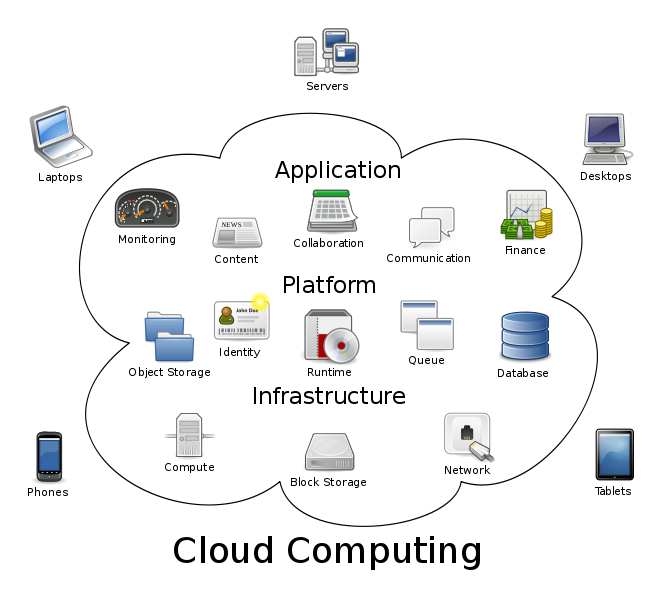
\includegraphics[scale=0.5]{images/662px-Cloud_computing.png}
    \end{center}
    \caption{Model Cloud Computing}
    \label{fig:ccsam}
  \end{figure}

\section{Karakteristik Cloud Computing}

Menurut NIST, ada beberapa karakteristik dari Cloud Computing:\index{Cloud Computing!Karakteristik}
\begin{itemize}
  \item \textbf{On-demand self-service}: layanan bisa diperoleh pada saat diminta, tanpa intervensi atau interaksi manusia di sisi penyedia jasa. 
  \item \textbf{Broad network access}: tersedia melalui jaringan dengan berbagai peranti yang umum (komputer, tablet, HP, dan lain-lain)
  \item \textbf{Resource pooling}: sumber daya komputasi dari penyedia jasa terkumpul untuk melayani.
  \item \textbf{Rapid elasticity}: skalabilitas.
  \item \textbf{Measured service}: penggunaan sumber daya bisa diukur, di-monitor, dikendalikan, dan dilaporkan.
\end{itemize}

Karakteristik lain yang tidak kalah penting adalah \textit{multitenancy}. \textit{Multitenancy} merupakan suatu prinsip dalam arsitektur software. Pada arsitektur tersebut, satu instan dari software berjalan pada server, melayani banyak organisasi klien. Aplikasi dirancang untuk mempartisi data dan konfigurasinya secara virtual dan setiap organisasi klien tersebut bekerja dengan instan aplikasi virtual tersebut\footnote{\url{http://en.wikipedia.org/wiki/Multitenancy}}. \index{Multitenancy}

\section{\textit{Public} dan \textit{Private} Cloud Computing}

\index{Cloud Computing!Private}Cloud Computing bisa dibangun untuk keperluan pribadi suatu organisasi dan (secara legal) hanya bisa diakses oleh organisasi yang bersangkutan. Tipe tersebut dikenal dengan \textit{Private Cloud Computing}. \index{Cloud Computing!Public}Sementara itu, jika sumber daya Cloud Computing bisa diakses oleh publik (dengan hak akses yang sesuai), maka model tersebut dikenal sebagai \textit{Public Cloud Computing}. Pembahasan di buku ini adalah pembahasan tentang \textit{Public Cloud Computing} dan semua referensi tentang Cloud Computing di buku ini akan menunjuk pada \textit{Public Cloud Computing} kecuali dinyatakan lain.

\section{Model Layanan Cloud Computing}

\index{Cloud Computing!Model layanan}Model layanan pada Cloud Computing akan berkembang sesuai kebutuhan konsumen serta inovasi dari berbagai penyedia layanan. Saat ini, pada umumnya, ada tiga model layanan:
\begin{itemize}
  \item \textbf{SaaS} (\textit{Software as a Service}): layanan berupa aplikasi yang ditempatkan pada infrastruktur penyedia layanan, siap digunakan oleh konsumen.
  \item \textbf{PaaS} (\textit{Platform as a Service}): menyediakan layanan ke konsumen berupa platform untuk men-deploy aplikasi.
  \item \textbf{IaaS} (\textit{Infrastructure as a Service}): menyediakan layanan ke konsumen berupa berbagai sumber daya komputasi (pemrosesam, penyimpanan, jaringan, dan sumber daya fundamental lainnya).
\end{itemize}

Meski sampai saat ini, umumnya terdapat tiga model tersebut, beberapa model kelihatannya sudah mulai muncul, misalnya STaaS (\textit{Storage as a Service}), SECaaS (\textit{Security as a Service}), DaaS (\textit{Data as a Service}), TEaaS (\textit{Test Environment as a Service}), \textit{Desktop Virtualization}, APIaaS (\textit{API as a Service}).

\section{Pengembangan Aplikasi di Cloud Computing}

Pada umumnya, para pengembang aplikasi di Cloud Computing juga menggunakan pendekatan \textit{Agile Software Development} yang berbasis pada pengembangan secara iteratif untuk setiap \textit{milestone} (dalam iterasi analisis-desain-\textit{coding-testing-debugging}) mulai dari \textit{milestone} paling awal sampai software dirilis. Perbedaan paling mendasar hanyalah pada platform yang digunakan untuk \textit{deployment}, peranti pengembangan yang digunakan, serta utilitas untuk mengelola aplikasi yang di-\textit{deploy} pada instan di cloud.

Pengembangan aplikasi di Cloud Computing akan melibatkan peranti pengembang yang didukung oleh infrastruktur Cloud. Kita akan memerlukan PaaS untuk keperluan ini. Pada dasarnya pengembangan aplikasi akan meliputi siklus berikut:

\begin{itemize}
  \item \textit{Coding}
  \item Test di komputer lokal
  \item Upload ke server (dalam Cloud Computing, proses ini diistilahkan dengan ``\textit{push}''
  \item Edit - push
\end{itemize}

Jika pengembangan aplikasi dilakukan oleh tim, maka perlu adanya software untuk \textit{version control}, misalnya Git, mercurial, dan lain-lain. Setelah itu, aktivitas yang dilakukan biasanya terpusat pada \textit{push} (untuk mengupload instan dari aplikasi ke server) dan \textit{pull} (untuk mengambil instan aplikasi dari server).

\section{Node.js dan Cloud Computing}

\index{Node.js}Node.js merupakan salah satu peranti pengembang yang bisa digunakan untuk membuat aplikasi berbasis Cloud. Node.js dikembangkan dari \textit{engine} JavaScript yang dibuat oleh Google untuk browser \textit{Chrome / Chromium} (V8) ditambah dengan libUV serta beberapa pustaka internal lainnya. Dengan menggunakan Node.js, semua pengembangan akan dilakukan menggunakan JavaScript, baik pada sisi klien maupun server. Node.js dibuat pertama kali oleh Ryan Dahl (twitter.com/ryah) dan sampai saat ini dikembangkan oleh komunitas sebagai software bebas dengan pendanaan utama dari Joyent, perusahaan tempat Ryan Dahl bekerja.

\section{Layanan Hosting Aplikasi: CloudFoundry}

\index{CloudFoundry}Saat ini, mulai banyak penyedia layanan Cloud yang mendukung Node.js, diantaranya adalah CloudFoundry (\url{http://www.cloudfoundry.com}, selanjutnya akan kita sebut dengan CF). Buku ini akan menggunakan fasilitas dari CF. Daftar lengkap dari penyedia infrastruktur Node.js bisa dilihat pada \url{https://github.com/joyent/node/wiki/Node-Hosting}.\index{Node.js!Hosting}

\subsection{Pendaftaran}

Untuk menggunakan fasilitas dari CF, kita akan mendaftar lebih dahulu di URL \url{https://mycloudfoundry.com/signup} sepert yang terlihat pada Gambar~\ref{fig:cfsignup}.

\begin{figure}[t]
    \begin{center}
      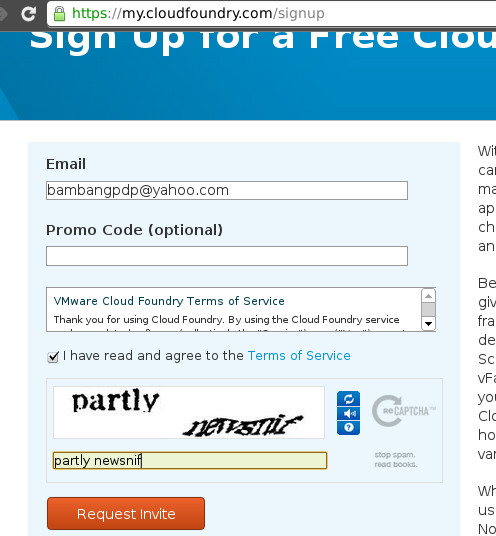
\includegraphics[scale=0.5]{images/cf-signup.jpg}
    \end{center}
    \caption{Pendaftaran di CF}
    \label{fig:cfsignup}
  \end{figure}

Setelah itu, CF akan mengirimkan pemberitahuan bahwa proses pendaftaran selesai seperti di Gambar~\ref{fig:cfsignuphasil}. \textit{Credentials} atau informasi tentang akun kita di CF akan dikirimkan ke e-mail kita seperti pada Gambar~\ref{fig:cfsignupapproved}.
 
  \begin{figure}
    \begin{center}
      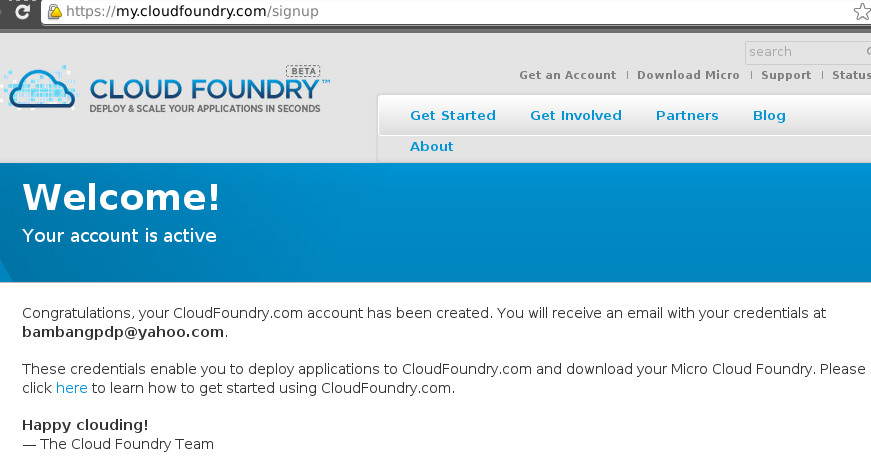
\includegraphics[scale=0.5]{images/cf-signup-hasil.jpg}
    \end{center}
    \caption{Hasil proses pendaftaran di CF}
    \label{fig:cfsignuphasil}
  \end{figure}

  \begin{figure}[t]
    \begin{center}
      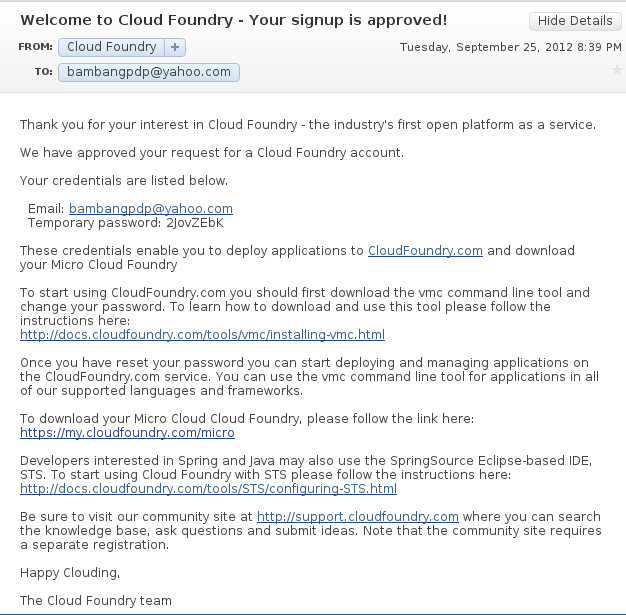
\includegraphics[scale=0.5]{images/cf-signup-approved.jpg}
    \end{center}
    \caption{E-mail persetujuan dan pemberitahuan \textit{credentials}}
    \label{fig:cfsignupapproved}
  \end{figure}

\subsection{Instalasi \textit{Command Line Utilities}}

\index{CloudFoundry!vmc}\textit{Command Line Utilities / CLU)} adalah software yang dijalankan melalui shell / \textit{command line / command prompt}. CLU untuk CF ini dibuat dengan menggunakan Ruby dan didistribusikan dalam bentuk \textit{gem} sehingga untuk instalasi ini diperlukan ruby dan rubygem. Berikut adalah perintah untuk instalasi vmc (CLU dari CF).

\lstset{language=bash,caption=Instalasi vmc}
\begin{lstlisting}
$ gem search vmc --remote | grep "\bvmc\s" 
vmc (0.4.7) 
$ gem install vmc 
Fetching: json_pure-1.6.7.gem (100%)
Fetching: interact-0.5.1.gem (100%)
Fetching: multipart-post-1.1.5.gem (100%)
Fetching: multi_json-1.4.0.gem (100%)
Fetching: rubyzip-0.9.9.gem (100%)
Fetching: cfoundry-0.4.17.gem (100%)
Fetching: clouseau-0.0.2.gem (100%)
Fetching: mothership-0.3.5.gem (100%)
Fetching: manifests-vmc-plugin-0.4.19.gem (100%)
Fetching: tunnel-dummy-vmc-plugin-0.0.2.gem (100%)
Fetching: vmc-0.4.7.gem (100%)
Successfully installed json_pure-1.6.7
Successfully installed interact-0.5.1
Successfully installed multipart-post-1.1.5
Successfully installed multi_json-1.4.0
Successfully installed rubyzip-0.9.9
Successfully installed cfoundry-0.4.17
Successfully installed clouseau-0.0.2
Successfully installed mothership-0.3.5
Successfully installed manifests-vmc-plugin-0.4.19
Successfully installed tunnel-dummy-vmc-plugin-0.0.2
Successfully installed vmc-0.4.7
11 gems installed
Installing ri documentation for json_pure-1.6.7...
Installing ri documentation for interact-0.5.1...
Installing ri documentation for multipart-post-1.1.5...
Installing ri documentation for multi_json-1.4.0...
Installing ri documentation for rubyzip-0.9.9...
Installing ri documentation for cfoundry-0.4.17...
Installing ri documentation for clouseau-0.0.2...
Installing ri documentation for mothership-0.3.5...
Installing ri documentation for manifests-vmc-plugin-0.4.19...
Installing ri documentation for tunnel-dummy-vmc-plugin-0.0.2...
Installing ri documentation for vmc-0.4.7...
Installing RDoc documentation for json_pure-1.6.7...
Installing RDoc documentation for interact-0.5.1...
Installing RDoc documentation for multipart-post-1.1.5...
Installing RDoc documentation for multi_json-1.4.0...
Installing RDoc documentation for rubyzip-0.9.9...
Installing RDoc documentation for cfoundry-0.4.17...
Installing RDoc documentation for clouseau-0.0.2...
Installing RDoc documentation for mothership-0.3.5...
Installing RDoc documentation for manifests-vmc-plugin-0.4.19...
Installing RDoc documentation for tunnel-dummy-vmc-plugin-0.0.2...
Installing RDoc documentation for vmc-0.4.7...
$
\end{lstlisting}

Hasil dari instalasi tersebut adalah sebagai berikut:

\lstset{language=bash,caption=Hasil gem yang terinstall}
\begin{lstlisting}
$ gem list 

*** LOCAL GEMS ***

bigdecimal (1.1.0)
cfoundry (0.4.17)
clouseau (0.0.2)
interact (0.5.1)
io-console (0.3)
json (1.5.4)
json_pure (1.6.7)
manifests-vmc-plugin (0.4.19)
minitest (2.5.1)
mothership (0.3.5)
multi_json (1.4.0)
multipart-post (1.1.5)
rake (0.9.2.2)
rdoc (3.9.4)
rubyzip (0.9.9)
tunnel-dummy-vmc-plugin (0.0.2)
vmc (0.4.7)
$ 
\end{lstlisting}

Setelah itu, tambahkan baris berikut di \textit{\$HOME/.bashrc} (catatan: "/home/bpdp/" adalah direktori \$HOME saya, silahkan sesuaikan dengan tempat anda):

\lstset{language=bash,caption=Mengaktifkan direktori "bin" hasil instalasi gem}
\begin{lstlisting}
export PATH=$PATH:/home/bpdp/.gem/ruby/1.9.1/bin
\end{lstlisting}

Periksa dengan menjalankan opsi help dari vmc:

\lstset{language=bash,caption=Hasil opsi help dari vmc}
\begin{lstlisting}
$ vmc help 
Showing basic command set. Pass --all to list all commands.

Getting Started
  login [USERNAME]	Authenticate with the target
  target [URL]    	Set or display the target cloud, organization, and space
  logout          	Log out from the target
  info            	Display information on the current target, user, etc.

Applications
  apps     	List your applications
  app [APP]	Show app information

  Management
    start APPS...  	Start an application
    delete APPS... 	Delete an application
    push [NAME]    	Push an application, syncing changes if it exists
    stop APPS...   	Stop an application
    restart APPS...	Stop and start an application

Services
  service INSTANCE	Show service instance information
  services        	List your service instances

  Management
    create-service [SERVICE] [NAME]	Create a service
    bind-service SERVICE APP       	Bind a service to an application
    unbind-service SERVICE APP     	Unbind a service from an application
    delete-service [INSTANCE]      	Delete a service
    tunnel [INSTANCE] [CLIENT]     	Tells you to install tunnel-vmc-plugin

Organizations
  create-org [NAME]        	Create an organization
  orgs                     	List available organizations
  delete-org [ORGANIZATION]	Delete an organization
  org [ORGANIZATION]       	Show organization information

Spaces
  create-space [NAME] [ORGANIZATION]	Create a space in an organization
  space [SPACE]                     	Show space information
  delete-space SPACES...            	Delete a space and its contents
  spaces [ORGANIZATION]             	List spaces in an organization

Routes
  create-route [URL]  	Create a route
  delete-route [ROUTE]	Delete a route
  routes              	List routes in a space

Domains
  create-domain NAME    	Create a domain
  delete-domain [DOMAIN]	Delete a domain
  add-domain NAME       	Add a domain to a space
  remove-domain [DOMAIN]	Remove a domain from a space
  domains [SPACE]       	List domains in a space

Options:
      --[no-]color       Use colorful output
      --[no-]script      Shortcut for --quiet and --force
  -V, --verbose          Print extra information
  -f, --[no-]force       Skip interaction when possible
  -h, --help             Show command usage & instructions
  -m, --manifest FILE    Path to manifest file to use
  -q, --[no-]quiet       Simplify output format
  -t, --trace            Show API requests and responses
  -u, --proxy EMAIL      Act as another user (admin only)
  -v, --version          Print version number
$ 
\end{lstlisting}

\subsection{Konfigurasi di Server Cloud}

Pada dasarnya, yang diperlukan hanyalah mengubah target ke server cloud dari CF dan kemudian mengubah password.

\lstset{language=bash,caption=Mengubah target server - belum ada konfigurasi}
\begin{lstlisting}
$ vmc target 
Errno::ENOENT: No such file or directory - /home/bpdp/.vmc/target
For more information, see ~/.vmc/crash
$
\end{lstlisting}

Error di atas terjadi karena file konfigurasi belum dibuat. File konfigurasi tersimpan di direktori \$HOME/.vmc. Mengubah target dilakukan dengan membuat file \textit{target} di direktori tersebut. Isi dari file target tersebut adalah server CloudFoundry, yaitu \textit{https://api.cloudfoundry.com}. Setelah itu, jika dieksekusi lagi, hasilnya adalah sebagai berikut:

\lstset{language=bash,caption=Mengubah target server - setelah konfigurasi}
\begin{lstlisting}
$ vmc target 
 
target: https://api.cloudfoundry.com

$ 
\end{lstlisting}

Setelah itu, setiap kali kita akan melakukan berbagai proses yang melibatkan server ini, kita harus melakukan proses login terlebih dahulu:

\lstset{language=bash,caption=Login ke server}
\begin{lstlisting}
$ vmc login 
target: https://api.cloudfoundry.com

Email> bambangpdp@yahoo.com

Password> ***************

Authenticating... OK

$ vmc info --all
Getting runtimes... OK
Getting frameworks... OK
Getting services... OK

VMware's Cloud Application Platform

target: https://api.cloudfoundry.com
  version: 0.999
  support: http://support.cloudfoundry.com

user: bambangpdp@yahoo.com

runtime   description
java      1.6.0_24   
java7     1.7.0_04   
node      0.4.12     
node06    0.6.8      
node08    0.8.2      
ruby18    1.8.7p357  
ruby19    1.9.2p180  

framework    description
grails       
java_web     
lift         
node         
play         
rack         
rails3       
sinatra      
spring       
standalone   

service      version   provider   description                          
mongodb      2.0       core       MongoDB NoSQL store                  
mysql        5.1       core       MySQL database service               
postgresql   9.0       core       PostgreSQL database service (vFabric)
rabbitmq     2.4       core       RabbitMQ message queue               
redis        2.4       core       Redis key-value store service        
redis        2.2       core       Redis key-value store service        
redis        2.6       core       Redis key-value store service    

$ 
\end{lstlisting}

Untuk mengubah password:

\lstset{language=bash,caption=Mengubah password server}
\begin{lstlisting}
$ vmc passwd 
New Password> **************

Verify Password> **************

Changing password... OK
$
\end{lstlisting}

\subsection{Instalasi dan Konfigurasi Node.js di Komputer Lokal}

Node.js tersedia untuk Linux, Windows, Mac OS X, serta SunOS. Untuk versi Linux, kebanyakan distro sudah menyertakan paket Node.js, hanya saja ada banyak versi dari Node.js dan jika kita menggunakan manajemen paket dari distro Linux, kita hanya bisa menginstall 1 versi saja. Sebagai contoh, di Arch Linux, paket Node.js bisa diinstrall dengan perintah ``pacman -S nodejs'' tetapi hanya pada versi resmi di repo Arch Linux (versi 0.8.16 pada tanggal 7 Januari 2012). 

Langkah instalasi berikut ini adalah langkah untuk instalasi tanpa manajemen paket dari distro Linux.
\begin{itemize}
  \item Ambil paket \textit{binary executable} dari \url{http://nodejs/download} atau langsung ke \url{http://nodejs.org/dist/}. Versi yang digunakan disini adalah 0.8.16. Download file tersebut, kemudian simpan di direktori tertentu (terserah anda, dibuku ini diletakkan di \$HOME/master/nodejs).

\lstset{language=bash,caption=Hasil dari download Node.js}
\begin{lstlisting}
$ ls -la
...
...
-rw-r--r--  1 bpdp users 4406113 Dec 13 06:16 node-v0.8.16-linux-x86.tar.gz
...
...
$ 
\end{lstlisting}

  \item Ekstrak ke direktori yang diinginkan. Node.js akan diinstall di direktori \$HOME/software:

\lstset{language=bash,caption=Ekstraksi Node.js}
\begin{lstlisting}
$ cd 
$ cd software
$ tar -xzvf ~/master/nodejs/node-v0.8.16-linux-x86.tar.gz
$ ln -s node-v0.8.16-linux-x86 nodejs
$ ls -la
....
....
lrwxrwxrwx   1 bpdp users    22 Dec 14 23:45 nodejs -> node-v0.8.16-linux-x86
drwxr-xr-x   6 bpdp users  4096 Dec 13 06:16 node-v0.8.16-linux-x86
....
....
$ 
\end{lstlisting}

  \item Konfigurasi variabel lingkungan. Sebaiknya disimpan pada suatu file (pada buku ini, konfigurasi akan disimpan di \textit{\$HOME/environment/nodejs}):

\lstset{language=bash,caption=Konfigurasi variabel lingkungan Node.js}
\begin{lstlisting}
NODEJS_HOME=/home/bpdp/software/nodejs
 
PATH=$PATH:$NODEJS_HOME/bin
MANPATH=$MANPATH:$NODEJS_HOME/share/man
LD_LIBRARY_PATH=$LD_LIBRARY_PATH:$NODEJS_HOME/lib
C_INCLUDE_PATH=$C_INCLUDE_PATH:$NODEJS_HOME/include
CPLUS_INCLUDE_PATH=$CPLUS_INCLUDE_PATH:$NODEJS_HOME/include
 
export PATH
export MANPATH
export LD_LIBRARY_PATH
export C_INCLUDE_PATH
export CPLUS_INCLUDE_PATH
\end{lstlisting}

  \item Setiap akan menggunakan Node.js, yang diperlukan adalah men-source file konfigurasi tersebut: \textbf{source \~/environment/nodejs}.
\end{itemize}

\section{Pengelolaan Aplikasi di Cloud}

Aplikasi yang dibuat nantinya akan di-deploy ke server CF. Pada umumnya, developer akan melakukan proses untuk upload (\textit{push}), menghapus (\textit{delete}), serta memperbaharui (\textit{update}) aplikasi di server. Jika belum memahami sintaksis JavaScript serta penggunaan npm, jangan kuatir. Tujuan dari bab ini hanya mengenalkan pengelolaan aplikasi di Cloud. Aspek lainnya akan dibahas di bab-bab berikutnya.

\subsection{\textit{Push, Delete, Update} Aplikasi}

Pada pembahasan ini, akan diberikan contoh menggunakan dua kategori, yaitu dengan menggunakan \textit{framework} (ExpressJS - \url{http://expressjs.com}) serta tanpa menggunakan \textit{framework}.

\subsection{Menggunakan Framework ExpressJS}

\lstset{language=bash,caption=Instalasi ExpressJS menggunakan npm}
\begin{lstlisting}
$ npm install -g express
\end{lstlisting}

Jika berhasil, maka kita bisa menggunakan perintah \textit{express} untuk membuat rerangka aplikasi. Sintaksis penggunaan ExpressJS adalah sebagai berikut:

\lstset{language=bash,caption=Perintah express}
\begin{lstlisting}
$ express --help

  Usage: express [options]

  Options:

    -h, --help          output usage information
    -V, --version       output the version number
    -s, --sessions      add session support
    -e, --ejs           add ejs engine support (defaults to jade)
    -J, --jshtml        add jshtml engine support (defaults to jade)
    -H, --hogan         add hogan.js engine support
    -c, --css <engine>  add stylesheet <engine> support (less|stylus) (defaults to plain css)
    -f, --force         force on non-empty directory

$
\end{lstlisting}

Setelah itu, kita bisa membuat rerangka aplikasi ExpressJS dengan cara berikut:

\lstset{language=bash,caption=Menggunakan express untuk membuat rerangka aplikasi}
\begin{lstlisting}
$ mkdir hello 
$ cd hello
$ express 

   create : .
   create : ./package.json
   create : ./app.js
   create : ./public
   create : ./public/images
   create : ./routes
   create : ./routes/index.js
   create : ./routes/user.js
   create : ./public/stylesheets
   create : ./public/stylesheets/style.css
   create : ./views
   create : ./views/layout.jade
   create : ./views/index.jade
   create : ./public/javascripts

   install dependencies:
     $ cd . && npm install

   run the app:
     $ node app

$
\end{lstlisting}

Pada rerangka aplikasi tersebut, terdapat file \textit{package.json} untuk mendefinisikan aplikasi serta dependensi-nya dan app.js yang merupakan file utama untuk dijalankan pada server.

\lstset{language=Javascript,caption=package.json untuk ExpressJS}
\begin{lstlisting}
{ 
  "name": "hello-node", 
  "version": "0.0.1", 
	"private": true,
	"scripts": {
		"start": "node app"
	},
  "dependencies":{ 
    "express": "3.0.6".
		"jade": "*"
  } 
} 
\end{lstlisting}

\lstset{language=Javascript,caption=app.js untuk ExpressJS}
\begin{lstlisting}
/**
 * Module dependencies.
 */

var express = require('express')
  , routes = require('./routes')
  , user = require('./routes/user')
  , http = require('http')
  , path = require('path');

var app = express();

app.configure(function(){
  app.set('port', process.env.PORT || 3000);
  app.set('views', __dirname + '/views');
  app.set('view engine', 'jade');
  app.use(express.favicon());
  app.use(express.logger('dev'));
  app.use(express.bodyParser());
  app.use(express.methodOverride());
  app.use(app.router);
  app.use(express.static(path.join(__dirname, 'public')));
});

app.configure('development', function(){
  app.use(express.errorHandler());
});

app.get('/', routes.index);
app.get('/users', user.list);

http.createServer(app).listen(app.get('port'), function(){
  console.log("Express server listening on port " + app.get('port'));
});
\end{lstlisting}

Edit file \textit{routes/index.js} sebagai berikut:

\lstset{language=Javascript,caption=Hasil edit routes/index.js}
\begin{lstlisting}
/*
 * GET home page.
 */

exports.index = function(req, res){
  res.render('index', { title: 'Express app at CloudFoundry' });
};
\end{lstlisting}

Setelah itu, install modul-modul yang diperlukan dengan perintah \textit{npm install} pada direktori tersebut. npm akan membaca file package.json kemudian menginstall modul-modul sesuai dengan deskripsi pada \textit{dependencies}. Setelah diuji pada komputer lokal dengan perintah \textit{node app}, dan sukses bisa diakses di browser dengan alamat \textit{http://localhost:3000}, maka aplikasi tersebut bisa di-deploy di CloudFoundry. Proses deployment digambarkan sebagai berikut (anda sudah harus login menggunakan perintah \textit{vmc login} sebelumnya) dan berada di direktori tempat aplikasi tersebut berada:

\lstset{language=bash,caption=Deployment aplikasi ExpressJS ke CF}
\begin{lstlisting}
$ vmc push
Name> hello-express

Instances> 1

1: node
2: other
Framework> node

1: node
2: node06
3: node08
4: other
Runtime> 3

1: 64M
2: 128M
3: 256M
4: 512M
5: 1G
Memory Limit> 64M

Creating hello-express... OK

1: hello-express.cloudfoundry.com
2: none
URL> hello-express.cloudfoundry.com

Updating hello-express... FAILED
The URI: "hello-express.cloudfoundry.com" has already been taken or reserved

1: hello-express.cloudfoundry.com
2: none
URL> bpdp-hello-express.cloudfoundry.com

Updating hello-express... OK

Create services for application?> n

Save configuration?> n

Uploading hello-express... OK
Starting hello-express... OK
Checking hello-express... OK

$ 
\end{lstlisting}

Hasilnya terlihat pada tampilan browser di Gambar~\ref{fig:modul1-hello}

  \begin{figure}
    \begin{center}
      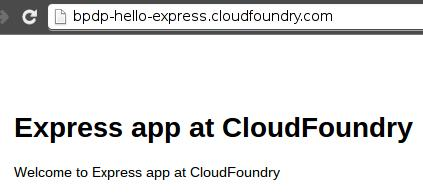
\includegraphics[scale=0.5]{images/bpdp-hello-express.jpg}
    \end{center}
    \caption{Hasil push ke server}
    \label{fig:modul1-hello}
  \end{figure}

Aplikasi yang sudah dibuat seringkali diubah, oleh karena itu vmc juga menyediakan fasilitas untuk Mengupdate aplikasi. 

\lstset{language=Javascript,caption=Update: menambahkan versi Node.js ke routes/index.js}
\begin{lstlisting}
/*
 * GET home page.
 */

exports.index = function(req, res){
	var nv = process.version;
  res.render('index', { title: 'Express app at CloudFoundry with Node.js ' + nv });
};
\end{lstlisting}

\lstset{language=bash,caption=Mengupdate aplikasi di server}
\begin{lstlisting}
$ vmc apps
Getting applications... OK

name              status    usage     runtime   url                                      
hello-express     running   1 x 64M   node08    bpdp-hello-express.cloudfoundry.com      
$ vmc push hello-express
Uploading hello-express... OK
Stopping hello-express... OK

Starting hello-express... OK
Checking hello-express... OK
$ 
\end{lstlisting}

Hasilnya bisa dilihat di Gambar~\ref{fig:modul1-hello-update}

  \begin{figure}
    \begin{center}
      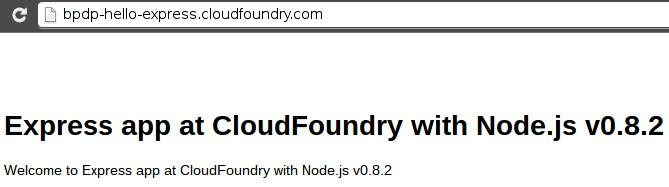
\includegraphics[scale=0.5]{images/bpdp-hello-express-update.jpg}
    \end{center}
    \caption{Hasil update dengan menyertakan versi Node.js}
    \label{fig:modul1-hello-update}
  \end{figure}

Untuk menghapus aplikasi:

\lstset{language=bash,caption=Menghapus aplikasi yang di-deploy di CF}
\begin{lstlisting}
$ vmc delete bpdp-m1-hellonoframework
Really delete bpdp-m1-hellonoframework?> y

Deleting bpdp-m1-hellonoframework... OK

$ 
\end{lstlisting}

Pada saat deployment, kita juga bisa memilih versi Node.js (runtime) sebagai berikut:

\lstset{language=bash,caption=Deployment ke CF dengan memilih runtime Node.js}
\begin{lstlisting}
$ vmc push --runtime=node08 
Name> bpdp-hello-express06

Instances> 1

1: node
2: other
Framework> node

1: 64M
2: 128M
3: 256M
4: 512M
5: 1G
Memory Limit> 64M

Creating bpdp-hello-express06... OK

1: bpdp-hello-express06.cloudfoundry.com
2: none
URL> bpdp-hello-express06.cloudfoundry.com

Updating bpdp-hello-express06... OK

Create services for application?> n

Save configuration?> n

Uploading bpdp-hello-express06... OK
Starting bpdp-hello-express06... OK
Checking bpdp-hello-express06... OK
$
\end{lstlisting}

Hasilnya bisa dilihat di Gambar~\ref{fig:modul1-hello-ganti-runtime}

  \begin{figure}
    \begin{center}
      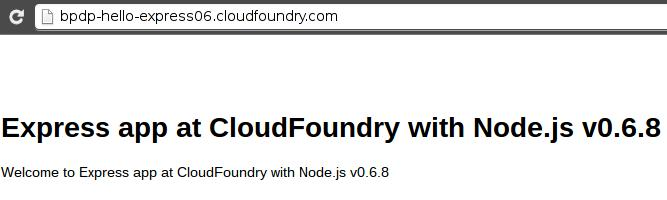
\includegraphics[scale=0.5]{images/bpdp-express-hello-update06.jpg}
    \end{center}
    \caption{Deployement menggunakan versi runtime tertentu}
    \label{fig:modul1-hello-ganti-runtime}
  \end{figure}

\subsection{Tanpa Framework}

Tanpa \textit{framework}, yang kita perlukan hanyalah langsung mem-\textit{push} file yang kita buat (dalam contoh ini adalah app.js):

\lstset{language=Javascript,caption=app.js tanpa framework}
\begin{lstlisting}

var http = require('http'); 
var url = require("url"); 

http.createServer(function (req, res) { 

    var pathname = url.parse(req.url).pathname; 

    res.writeHead(200, {'Content-Type': 'text/html'}); 
    res.write("Hello NodeJS <u>" + process.version + "</u>"); 
    res.write("<br />Request for <b>" + pathname + "</b> received."); 
    res.end(); 

}).listen(1337);
\end{lstlisting}

Proses deployement adalah sebagai berikut:

\lstset{language=bash,caption=Deployment app.js tanpa framework}
\begin{lstlisting}
$ vmc push
Name> hello-noframework

Instances> 1

1: node
2: other
Framework> node

1: node
2: node06
3: node08
4: other
Runtime> 3

1: 64M
2: 128M
3: 256M
4: 512M
5: 1G
Memory Limit> 64M

Creating hello-noframework... OK

1: hello-noframework.cloudfoundry.com
2: none
URL> hello-noframework.cloudfoundry.com

Updating hello-noframework... OK

Create services for application?> n

Save configuration?> n

Uploading hello-noframework... OK
Starting hello-noframework... OK
Checking hello-noframework... OK
$
\end{lstlisting}

Hasilnya bisa dilihat pada Gambar~\ref{fig:modul1-hello-no-framework}

  \begin{figure}
    \begin{center}
      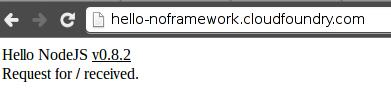
\includegraphics[scale=0.5]{images/hello-noframework.jpg}
    \end{center}
    \caption{Hasil deployement app.js tanpa framework}
    \label{fig:modul1-hello-no-framework}
  \end{figure}

 \chapter{REPL dan Dasar-dasar JavaScript di Node.js}

\section{REPL}

REPL adalah lingkungan pemrograman interaktif, tempat developer bisa mengetikkan program per baris dan langsung mengeksekusi hasilnya. Biasanya ini digunakan untuk menguji perintah-perintah yang cukup dijalankan pada satu baris atau satu blok segmen kode sumber saja. Karena fungsinya itu, maka istilah yang digunakan adalah REPL (read-eval-print-loop), yaitu loop atau perulangan baca perintah - evaluasi perintah - tampilkan hasil. REPL sering juga disebut sebagai \textit{interactive top level} atau \textit{language shell}. ``Tradisi'' ini sudah dimulai sejak jaman LISP di mesin UNIX di era awal pengembangan \textit{development tools}. Saat ini hampir semua \textit{interpreter/compiler} mempunyai REPL, misalnya Python, Ruby, Scala, PHP, berbagai interpreter/compiler LISP, dan tidak ketinggalan Node.js. 

\subsection{Mengaktifkan REPL}

Untuk mengaktifkan REPL dari Node.js, \textit{executable command line program}-nya adalah \textbf{node}. Jika \textbf{node} dipanggil dengan argumen nama file JavaScript, maka file JavaScript tersebut akan dieksekusi, sementara jika tanpa argumen, akan masuke ke REPL:

\lstset{language=bash,caption=Node.js REPL}
\begin{lstlisting}
$ node
> .help
.break	Sometimes you get stuck, this gets you out
.clear	Alias for .break
.exit	Exit the repl
.help	Show repl options
.load	Load JS from a file into the REPL session
.save	Save all evaluated commands in this REPL session to a file
>
\end{lstlisting}

Tanda ``\textbf{>}'' adalah tanda bahwa REPL Node.js siap untuk menerima perintah. Untuk melihat perintah-perintah REPL, bisa digunakan \textbf{.help}.

\subsection{Perintah-perintah REPL}

Pada sesi REPL, kita bisa memberikan perintah internal REPL maupun perintah-perintah lain yang sesuai dan dikenali sebagai perintah JavaScript. Perintah internal REPL Node.js terdiri atas:
\begin{itemize}
  \item \textbf{.break}: keluar dan melepaskan diri dari "keruwetan" baris perintah di REPL.
  \item \textbf{.clear}: alias untuk .break
  \item \textbf{.exit}: keluar dari sesi REPL (bisa juga dengan menggunakan Ctrl-D)
  \item \textbf{.help}: menampilkan pertolong perintah internal REPL
  \item \textbf{.load}: membaca dan mengeksekusi perintah-perintah JavaScript yang terdapat pada suatu file.
  \item \textbf{.save}: menyimpan sesi REPL ke dalam suatu file.
\end{itemize}

Contoh untuk \textbf{.load}:

\lstset{language=JavaScript,caption=Contoh penggunaan .load dalam REPL}
\begin{lstlisting}
> .load /home/bpdp/kerjaan/src/javascript/nodejs/server.js
> var http = require('http');
undefined
> http.createServer(function (req, res) {
...     res.writeHead(200, {'Content-Type': 'text/plain'});
...       res.end('Hello, world!\n');
... }).listen(8124, "127.0.0.1");
{ _connections: 0,
  connections: [Getter/Setter],
  allowHalfOpen: true,
  _handle: null,
  _events: 
   { request: [Function],
     connection: [Function: connectionListener] },
  httpAllowHalfOpen: false }
> console.log('Server running at http://127.0.0.1:8124/');
Server running at http://127.0.0.1:8124/
undefined
>
\end{lstlisting}

Setelah keluar dari sesi REPL, maka port akan ditutup dan hasil eksekusi di atas akan dibatalkan. 

Untuk menyimpan hasil sesi REPL menggunakan \textbf{.save}, jika tanpa menyebutkan direktori, maka akan disimpan di direktori aktif saat itu. Contoh:
\lstset{language=bash,caption=Contoh penggunaan perintah .save di sesi REPL}
\begin{lstlisting}
$ node
> console.log("Selamat datang di Node.js")
Selamat datang di Node.js
undefined
> .save /home/bpdp/kerjaan/src/javascript/nodejs/hello.js
Session saved to:/home/bpdp/kerjaan/src/javascript/nodejs/hello.js
> [bpdp@bpdp-arch ~]$ cat /home/bpdp/kerjaan/src/javascript/nodejs/hello.js 
console.log("Selamat datang di Node.js")
\end{lstlisting}

\section{Dasar-dasar JavaScript di Node.js}

Node.js merupakan sistem peranti lunak yang merupakan implementasi dari bahasa pemrograman JavaScript. Spesifikasi JavaScript yang diimplementasikan merupakan spesifikasi resmi dari ECMAScript serta CommonJS (\url{http://commonjs.org}). Dengan demikian, jika anda sudah pernah mempelajari JavaScript sebelumnya, tata bahasa dari perintah yang dipahami oleh Node.js masih tetap sama dengan JavaScript. 

\subsection{Membaca \textit{Masukan} dari Stream / Masukan Standar (stdin)}

Untuk lebih memahami dasar-dasar JavaScript serta penerapannya di Node.js, seringkali kita perlu melakukan simulasi pertanyaan - proses - keluaran jawaban. Proses akan kita pelajari seiring dengan materi-materi berikutnya, sementara untuk keluaran, kita bisa menggunakan \textbf{console.log}. Bagian ini akan menjelaskan sedikit tentang masukan.

Perintah untuk memberi masukan di Node.js sudah tersedia pada pustaka API \textit{Readline}\footnote{Lengkapnya bisa diakses di \url{http://nodejs.org/api/readline.html}}. Pola dari masukan ini adalah sebagai berikut:
\begin{itemize}
  \item me-\textit{require} pustaka Readline
  \item membuat \textit{interface} untuk masukan dan keluaran
  \item .. gunakan interface ..
  \item .. gunakan interface ..
  \item .. gunakan interface ..
  \item .. gunakan interface ..
  \item ..
  \item ..
  \item tutup \textit{interface}
\end{itemize}

Implementasi dari pola diatas bisa dilihat pada kode sumber berikut ini (diambil dari manual Node.js):

\lstset{language=JavaScript,caption=readline.js: penggunaan pustaka Readline untuk masukan}
\begin{lstlisting}
var readline = require('readline');

var rl = readline.createInterface({
  input: process.stdin,
  output: process.stdout
});

rl.question("What do you think of node.js? ", function(answer) {
  console.log("Thank you for your valuable feedback:", answer);

  rl.close();
});
\end{lstlisting}

Hasilnya adalah sebagai berikut:

\lstset{language=bash,caption=Hasil eksekusi readline.js}
\begin{lstlisting}
[bpdp@bpdp-arch modul-2]$ node readline.js 
What do you think of node.js? awesome!
Thank you for your valuable feedback: awesome!
[bpdp@bpdp-arch modul-2]$
\end{lstlisting}


\begin{Sbox}
\begin{minipage}{\textwidth}
\textbf{Catatan:} \textit{function(answer)} pada listing di atas merupakan \textit{anonymous function} atau fungsi anonimus (sering juga disebut \textit{lambda function} / fungsi lambda. Posisi fungsi pada listing tersebut disebut dengan fungsi \textit{callback}. Untuk keperluan pembahasan saat ini, untuk sementara yang perlu dipahami adalah hasil input akan dimasukkan ke \textit{answer} untuk diproses lebih lanjut. Fungsi dan \textit{callback} akan dibahas lebih lanjut pada pembahasan berikutnya.
\end{minipage}
\end{Sbox}
\begin{center}
\shadowbox{\TheSbox}
\end{center}

\subsection{Nilai/Value dan Tipe Data}

Program dalam JavaScript akan berhubungan dengan data atau nilai. Setiap nilai mempunyai tipe tertentu. JavaScript mengenali berbagai tipe berikut ini:
\begin{itemize}
  \item Angka: bulat (misalnya 4) atau pecahan (misalnya 3.75)
  \item \textit{Boolean}: nilai benar (true) dan salah (false)
  \item String: diapit oleh tanda petik ganda ("contoh string") atau tunggal ('contoh string')
  \item \textit{null}
  \item \textit{undefined}
\end{itemize}

JavaScript adalah bahasa pemrograman yang mengijinkan pemrogram untuk tidak mendefinisikan tipe data pada saat deklarasi, atau sering juga disebut sebagai \textit{dynamically typed language}:

\lstset{language=JavaScript,caption=Fitur \textit{dynamically typed language}}
\begin{lstlisting}
var jumlahMahasiswa = 30
console.log('Jumlah mahasiswa dalam satu kelas = ' + jumlahMahasiswa);
// Jumlah mahasiswa dalam satu kelas = 30
\end{lstlisting} 

Pada contoh di atas, kita bisa melihat bahwa data akan dikonversi secara otomatis pada saat program dieksekusi.

\begin{Sbox}
\begin{minipage}{\textwidth}
\textbf{Catatan:}
\begin{itemize}
  \item Khusus untuk operator "+", JavaScript akan melakukan penggabungan string (\textit{string concatenation}), tetapi untuk operator lain, akan dilakukan operasi matematis sesuai operator tersebut (-,/,*).
  \item Konversi string ke tipe numerik bisa dilakukan dengan \textit{parseInt(string)} (jika bilangan bulat) dan \textit{parseFloat(string)} (jika bilangan pecahan).
\end{itemize}
\end{minipage}
\end{Sbox}
\begin{center}
\shadowbox{\TheSbox}
\end{center}

\subsection{Variabel}

Variabel adalah suatu nama yang didefinisikan untuk menampung suatu nilai. Nama ini akan digunakan sebagai referensi yang akan menunjukkan ke nilai yang ditampungnya. Nama variabel disebut dengan \textit{identifier} / pengenal. Ada beberapa syarat pemberian nama \textit{identifier} di JavaScript: 
\begin{itemize}
  \item Dimulai dengan huruf, \textit{underscore} (\_), atau tanda dollar (\$).
  \item Karakter berikutnya bisa berupa angka, selain ketentuan pertama di atas.
  \item Membedakan huruf besar - kecil.
\end{itemize}
Konvensi yang digunakan oleh pemrogram JavaScript terkait dengan penamaan ini adalah variasi dari metode \textit{camel case}, yaitu \textit{camelBack}. Contoh: jumlahMahasiswa, linkMenu, status.

\subsection{Konstanta}

Konstanta mirip dengan variabel, hanya saja sifatnya \textit{read-only}, tidak bisa diubah-ubah setelah ditetapkan. Untuk menetapkan konstanta di JavaScript, digunakan kata kunci \textit{const}. Contoh: 

\lstset{language=JavaScript,caption=Contoh konstanta dalam JavaScript}
\begin{lstlisting}
const DEFAULT\_MENU = ``Home'';
\end{lstlisting}

Konvensi penamaan konstanta adalah menggunakan huruf besar semua. Bagian ini (sampai saat buku ini ditulis) hanya berlaku di Firefox dan Google Chrome - V8 (artinya berlaku juga untuk Node.js).

\subsection{Fungsi}

\subsubsection{Pengertian Fungsi}

Fungsi merupakan subprogram atau suatu bagian dari keseluruhan program yang ditujukan untuk mengerjakan suatu pekerjaan tertentu dan (biasanya) menghasilkan suatu nilai kembalian. Subprogram ini relatif independen terhadap bagian-bagian lain sehingga memenuhi kaidah "bisa-digunakan-kembali" atau \textit{reusable} pada beberapa program yang memerlukan fungsionalitasnya. Fungsi dalam ilmu komputer sering kali juga disebut dengan \textit{prcedure, routine}, atau \textit{method}.

\subsubsection{Definisi Fungsi}

Definisi fungsi dari JavaScript di Node.js bisa dilakukan dengan sintaksis berikut ini:

\lstset{language=JavaScript,caption=Sintaksis Fungsi dalam JavaScript}
\begin{lstlisting}
function namaFungsi(argumen1, argumen2, ... , argumentN) {
  ..
  JavaScript code ..
  JavaScript code ..
  JavaScript code ..
  JavaScript code ..
  ..
}
\end{lstlisting}

Setelah dideklarasikan, fungsi tersebut bisa dipanggil dengan cara sebagai berikut:

\lstset{language=JavaScript,caption=Pemanggilan Fungsi dalam JavaScript}
\begin{lstlisting}
..
..
  namaFungsi(argumen1, argumen2, ..., argumenN);
..
..
\end{lstlisting}

Contoh dalam program serta pemanggilannya adalah sebagai berikut:

\lstset{language=bash,caption=Contoh deklarasi fungsi dan pemanggilannya}
\begin{lstlisting}
$ node
> function addX(angka) {
... console.log(angka + 10);
... }
undefined
> addX(20);
30
undefined
>
> function add2Numbers(angka1, angka2) {
... return angka1 + angka2;
... }
undefined
> console.log("232 + 432 = " + add2Numbers(232, 432));
232 + 432 = 664
undefined
>
\end{lstlisting}

\subsubsection{Fungsi Anonim}

Fungsi anonim adalah fungsi tanpa nama, pemrogram tidak perlu memberikan nama ke fungsi. Biasanya fungsi anonimus ini hanya digunakan untuk fungsi yang dikerjakan pada suatu bagian program saja dan tidak dengan maksud untuk dijadikan komponen yang bisa dipakai di bagian lain dari program (biasanya untuk menangani \textit{event} atau \textit{callback}). Untuk mendeklarasikan fungsi ini, digunakan operator \textit{function}.

\lstset{language=JavaScript,caption=Fungsi anonim}
\begin{lstlisting}
var pangkat = function(angka) {return angka * angka};
console.log(pangkat(10));
// output: 100
\end{lstlisting}

\subsubsection{Fungsi Rekursif}

Fungsi rekursif adalah fungsi yang memanggil dirinya sendiri. Contoh dari aplikasi fungsi rekursif adalah pada penghitungan faktorial berikut:

\lstset{language=JavaScript,caption=Fungsi rekursif untuk menghitung faktorial}
\begin{lstlisting}
function factorial(n){
  if ((n == 0) || (n == 1))
    return 1;
  else
    return (n * factorial(n - 1));
}
\end{lstlisting}

\subsection{Literal}

Literal digunakan untuk merepresentasikan nilai dalam JavaScript. Ada beberapa tipe literal.

\subsubsection{Literal Array}

Array atau variabel berindeks adalah penampung untuk obyek yang menyerupai \textit{list} atau daftar. Obyek array juga menyediakan berbagai fungsi dan metode untuk mengolah anggota yang terdapat dalam daftar tersebut (terutama untuk operasi \textit{traversal} dan permutasi.

\subsubsection{Literal Boolean}


\subsubsection{Literal Integer}

\subsubsection{Literal Floating-point}

\subsubsection{Literal Obyek}

Literal ini akan dibahas di bab yang menjelaskan tentang paradigma pemrograman berorientasi obyek di JavaScript.

\subsubsection{Literal String}


\subsection{Aliran Kendali}

\subsection{Penanganan Error}

\subsection{Struktur Data dan Representasi JSON}


 \chapter{Paradigma Pemrograman di JavaScript}

\section{Pemrograman Fungsional}

Pemrograman fungsional, atau sering disebut \textit{functional programming}, selama ini lebih sering dibicarakan di level para akademisi. Meskipun demikian, saat ini terdapat kecenderungan paradigma ini semakin banyak digunakan di industri. Contoh nyata dari implementasi paradigma ini di industri antara lain adalah Scala (\url{http://www.scala-lang.org}), OCaml (\url{http://www.ocaml.org}), Haskell (\url{http://www.haskell.org}), Microsoft F\# (\url{http://fsharp.org}), dan lain-lain. Dalam konteks paradigma pemrograman, peranti lunak yang dibangun menggunakan pendekatan paradigma ini akan terdiri atas berbagai fungsi yang mirip dengan fungsi matematis. Fungsi matematis tersebut di-evaluasi dengan penekanan pada penghindaran \textit{state} serta \textit{mutable data}. Bandingkan dengan paradigma pemrograman prosedural yang menekankan pada \textit{immutable data} dan definisi berbagai prosedur dan fungsi untuk mengubah \textit{state} serta data.

JavaScript bukan merupakan bahasa pemrograman fungsional yang murni, tetapi ada banyak fitur dari pemrograman fungsional yang terdapat dalam JavaScript. Dalam hal ini, JavaScript banyak dipengaruhi oleh bahasa pemrograman Scheme (\url{http://www.schemers.org/}). Bab ini akan membahas beberapa fitur pemrograman fungsional di JavaScript. Pembahasan ini didasari pembahasan di bab sebelumnya tentang Fungsi di JavaScript.

\subsection{Ekspresi Lambda}

\index{Ekspresi Lambda}Ekspresi lambda / \textit{lambda expression} merupakan hasil karya dari ALonzo Church sekitar tahun 1930-an. Aplikasi dari konsep ini di dalam pemrograman adalah penggunaan fungsi sebagai parameter untuk suatu fungsi. Dalam pemrograman, \textit{lambda function} sering juga disebut sebagai fungsi anonimus (fungsi yang dipanggil/dieksekusi tanpa ditautkan (\textit{bound}) ke suatu \textit{identifier}). Berikut adalah implementasi dari konsep ini di JavaSCript:

\lstset{language=JavaScript,caption=Ekspresi Lambda di JavaScript}
\begin{lstlisting}
// Diambil dari 
// http://stackoverflow.com/questions/3865335/what-is-a-lambda-language
// dengan beberapa perubahan

function applyOperation(a, b, operation) {
	return operation(a, b);
}

function add(a, b) {
	return a+b;
}

function subtract(a, b) {
	return a-b;
}

console.log('1,2, add: ' + applyOperation(1,2, add));
console.log('43,21, subtract: ' + applyOperation(43,21, subtract));

console.log('4^3: ' + applyOperation(4, 3, function(a,b) {return Math.pow(a, b)}))

// hasil:
// 1,2, add: 3
// 43,21, subtract: 22
// 4^3: 64
\end{lstlisting}

\subsection{Higher-order Function}

\index{Higher-order Function}\textit{Higher-order function} (sering disebut juga sebagai \textit{functor} adalah suatu fungsi yang setidak-tidaknya menggunakan satu atau lebih fungsi lain sebagai parameter dari fungsi, atau menghasilkan fungsi sebagai nilai kembalian. 

\lstset{language=JavaScript,caption=Higher-order Function di JavaScript}
\begin{lstlisting}
function forEach(array, action) {
	for (var i = 0; i < array.length; i++ )
		action(array[i]);
}

function print(word) {
	console.log(word);
}

function makeUpperCase(word) {
	console.log(word.toUpperCase());
}

forEach(["satu", "dua", "tiga"], print);
forEach(["satu", "dua", "tiga"], makeUpperCase);

// hasil:
//satu
//dua
//tiga
//SATU
//DUA
//TIGA
\end{lstlisting}

\subsection{Closure}

\index{Closure}Suatu \textit{closure} merupakan definisi suatu fungsi bersama-sama dengan lingkungannya. Lingkungan tersebut terdiri atas fungsi internal serta berbagai variabel lokal yang masih tetap tersedia saat fungsi utama / closure tersebut selesai dieksekusi. 

\lstset{language=JavaScript,caption=Closure di JavaScript}
\begin{lstlisting}
// Diambil dengan sedikit perubahan dari:
// https://developer.mozilla.org/en-US/docs/JavaScript/Guide/Closures
function makeAdder(x) {
  return function(y) {
    return x + y;
  };
}
 
var add5 = makeAdder(5);
var add10 = makeAdder(10);
 
console.log(add5(2));  // 7
console.log(add10(2)); // 12
\end{lstlisting}

\subsection{Currying}

\index{Currying}\textit{Currying} memungkinkan pemrogram untuk membuat suatu fungsi dengan cara menggunakan fungsi yang sudah tersedia secara parsial, artinya tidak perlu menggunakan semua argumen dari fungsi yang sudah tersedia tersebut.

\lstset{language=JavaScript,caption=Currying di JavaScript}
\begin{lstlisting}
// Diambil dari:
// http://javascriptweblog.wordpress.com/2010/04/05/
// 		curry-cooking-up-tastier-functions/
// dengan sedikit perubahan

function toArray(fromEnum) {
    return Array.prototype.slice.call(fromEnum);
}

Function.prototype.curry = function() {
    if (arguments.length<1) {
        return this; //nothing to curry with - return function
    }
    var __method = this;
    var args = toArray(arguments);
    return function() {
        return __method.apply(this, args.concat(toArray(arguments)));
    }
}

var add = function(a,b) {
    return a + b;
}

//create function that returns 10 + argument
var addTen = add.curry(10); 
console.log(addTen(20)); //30
\end{lstlisting}


\section{Pemrograman Berorientasi Obyek}

\subsection{Pengertian}

\index{PBO}Pemrograman Berorientasi Obyek (selanjutnya akan disingkat PBO) adalah suatu paradigma pemrograman yang memandang bahwa pemecahan masalah pemrograman akan dilakukan melalui definisi berbagai kelas kemudian membuat berbagai obyek berdasarkan kelas yng dibuat tersebut dan setelah itu mendefinisikan interaksi antar obyek tersebut dalam memecahkan masalah pemrograman. Obyek bisa saling berinteraksi karena setiap obyek mempunyai properti (sifat / karakteristik) dan \textit{method} untuk mengerjakan suatu pekerjaan tertentu. Jadi, bisa dikatakan bahwa paradigma ini menggunakan cara pandang yang manusiawi dalam penyelesaian masalah.

Dengan demikian, inti dari PBO sebenarnya terletak pada kemampuan untuk mengabstraksikan berbagai obyek ke dalam kelas (yang terdiri atas properti serta method). Paradigma PBO biasanya juga mencakup \textit{inheritance} atau pewarisan (sehingga terbentuk skema yang terdiri atas \textit{superclass} dan \textit{subclass}). Ciri lainnya adalah \textit{polymorphism} dan \textit{encapsulation} / pengkapsulan.

JavaScript adalah bahasa pemrograman yang mendukung PBO dan merupakan implementasi dari ECMAScript. Implementasi PBO di JavaScript adalah \textit{prototype-based programming} yang merupakan salah satu subset dari PBO. Pada \textit{prototype-based programming}, kelas / \textit{class} tidak ada. Pewarisan diimplementasikan melalui \textit{prototype}.

\subsection{Definisi Obyek}

\index{Obyek}Definisi obyek dilakukan dengan menggunakan definisi \textit{function}, sementara \textit{this} digunakan di dalam definisi untuk menunjukkan ke obyek tersebut. Sementara itu, Kelas.prototype.namaMethod digunakan untuk mendefinisikan method dengan nama method namaMethod pada kelas Kelas. Perhatikan contoh pada listing berikut.

\lstset{language=JavaScript,caption=Definisi obyek di JavaScript}
\begin{lstlisting}
var url = require('url');

// Definisi obyek
function Halaman(alamatUrl) {
  this.url = alamatUrl;
  console.log("Mengakses alamat " + alamatUrl);
}

Halaman.prototype.getDomainName = function() {
  return url.parse(this.url, true).host; 
}
// sampai disini definisi obyek
// Halaman.prototype.getDomainName => menetapkan method getDomainName
// untuk obyek

var halSatu = new Halaman("http://nodejs.org/api/http.html");
var halDua = new Halaman("http://bpdp.name/login?fromHome");

console.log("Alamat URL yang diakses oleh halSatu = " + halSatu.url);
console.log("Alamat URL yang diakses oleh halDua = " + halDua.url);

console.log("Nama domain halDua = " + halDua.getDomainName());

// hasil:
// Mengakses alamat http://nodejs.org/api/http.html
// Mengakses alamat http://bpdp.name/login?fromHome
// Alamat URL yang diakses oleh halSatu = http://nodejs.org/api/http.html
// Alamat URL yang diakses oleh halDua = http://bpdp.name/login?fromHome
// Nama domain halDua = bpdp.name
\end{lstlisting}

\subsection{\textit{Inheritance} / Pewarisan}

\index{Pewarisan}Pewarisan di JavaScript bisa dicapai menggunakan \textit{prototype}. Listing program berikut memperlihatkan bagaimana pewarisan diimplementasikan di JavaScript.

\lstset{language=JavaScript,caption=Pewarisan di PBO JavaScript}
\begin{lstlisting}
// Definisi obyek
function Kelas(param) {
  this.property1 = new String(param);
}

Kelas.prototype.methodSatu = function() {
  return this.property1; 
}

var kelasSatu = new Kelas("ini parameter 1 dari kelas 1");

console.log("Property 1 dari kelasSatu = " + kelasSatu.property1);
console.log("Property 1 dari kelasSatu, diambil dari method  = " + kelasSatu.methodSatu());

// Definisi inheritance:
// SubKelas merupakan anak dari Kelas yang didefinisikan
// di atas.

SubKelas.prototype = new Kelas();
SubKelas.prototype.constructor = SubKelas;

function SubKelas(param) {
  this.property1 = new String(param);
}

// method overriding
SubKelas.prototype.methodSatu = function(keHurufBesar) {
  console.log("Ubah ke huruf besar? = " + keHurufBesar);
  if (keHurufBesar) {
    return this.property1.toUpperCase();
  } else {
    return this.property1.toLowerCase();
  }
}

SubKelas.prototype.methodDua = function() {
  console.log("Berada di method dua dari SubKelas");
}

// mari diuji
var subKelasSatu = new SubKelas("Parameter 1 Dari Sub Kelas 1");

console.log("Property 1 dari sub kelas 1 = " + subKelasSatu.property1);
console.log("Property 1 dari sub kelas 1, diambil dari method+param = " + 
  subKelasSatu.methodSatu(true));
console.log("Property 1 dari sub kelas 1, diambil dari method+param = " +
  subKelasSatu.methodSatu(false));

console.log(subKelasSatu.methodDua());
// hasil:
//
//Property 1 dari kelasSatu = ini parameter 1 dari kelas 1
//Property 1 dari kelasSatu, diambil dari method  = ini 
//parameter 1 dari kelas 1
//Property 1 dari sub kelas 1 = Parameter 1 Dari Sub Kelas 1
//Ubah ke huruf besar? = true
//Property 1 dari sub kelas 1, diambil dari method+param = 
//PARAMETER 1 DARI SUB KELAS 1
//Ubah ke huruf besar? = false
//Property 1 dari sub kelas 1, diambil dari method+param = 
//parameter 1 dari sub kelas 1
//Berada di method dua dari SubKelas
\end{lstlisting}

 \chapter{Mengelola Paket Menggunakan npm}

\section{Apakah npm Itu?}

\index{npm}Node.js memungkinkan developer untuk mengembangkan aplikasi secara modular dengan memisahkan berbagai komponen \textit{reusable code} ke dalam pustaka (\textit{library}). Berbagai pustaka tersebut bisa diperoleh di \url{http://npmjs.org}. Node.js menyediakan perintah \textit{npm} untuk mengelola paket pustaka di repositori tersebut. Untuk menggunakan utilitas ini, pemrogram harus terkoneksi dengan Internet.

\section{Menggunakan npm}

Saat melakukan instalasi Node.js, secara otomatis \textit{npm} akan disertakan. Dengan perintah \textit{npm} tersebut, seorang pemrogram bisa mengelola pustaka yang tersedia di repositori. Jika pemrogram mempunya pustakan yang bisa digunakan oleh orang lain, maka pemrogram yang bersangkutan juga bisa menyimpan pustaka tersebut ke dalam repositori sehingga memungkinkan untuk diinstall oleh pemrogram-pemrogram lain di seluruh dunia. Sintaksis lengkap dari penggunaan perintah \textit{npm} ini adalah sebagai berikut\footnote{beberapa bagian tertulis spesifik lokasi direktori di komputer yang digunakan penulis}:

\lstset{language=bash,caption=Sintaksis lengkap perintah \textit{npm}}
\begin{lstlisting}
$ npm --help

Usage: npm <command>

where <command> is one of:
    add-user, adduser, apihelp, author, bin, bugs, c, cache,
    completion, config, ddp, dedupe, deprecate, docs, edit,
    explore, faq, find, find-dupes, get, help, help-search,
    home, i, info, init, install, isntall, issues, la, link,
    list, ll, ln, login, ls, outdated, owner, pack, prefix,
    prune, publish, r, rb, rebuild, remove, restart, rm, root,
    run-script, s, se, search, set, show, shrinkwrap, star,
    stars, start, stop, submodule, tag, test, tst, un,
    uninstall, unlink, unpublish, unstar, up, update, version,
    view, whoami

npm <cmd> -h     quick help on <cmd>
npm -l           display full usage info
npm faq          commonly asked questions
npm help <term>  search for help on <term>
npm help npm     involved overview

Specify configs in the ini-formatted file:
    /home/bpdp/.npmrc
or on the command line via: npm <command> --key value
Config info can be viewed via: npm help config

npm@1.2.14 /home/bpdp/software/node-v0.10.0-linux-x86/lib/node_modules/npm
\end{lstlisting}

Pada bagian berikut, kita akan membahas lebih lanjut penggunaan perintah \textit{npm} tersebut.

\subsection{Instalasi Paket}

\index{npm!install paket}npm sebenarnya bukan merupakan singkatan dari \textit{Node Package Manager}, meskipun seringkali orang menterjemahkan dengan singkatan tersebut dan npm seharusnya ditulis dalam huruf kecil semua seperti yang dijelaskan pada FAQ (\textit{Frequently Asked Questions})\footnote{\url{https://npmjs.org/doc/faq.html}}. npm merupakan bilah alat berbasis baris perintah, dijalankan melalui shell atau \textit{command prompt}. Sama seperti kebanyakan bilah alat berbasis baris perintah lain, npm memiliki struktur perintah \textit{npm perintah argumen}. Installasi paket pustaka dilakukan dengan perintah berikut :

\lstset{language=bash,caption=Cara install paket menggunakan npm}
\begin{lstlisting}
$ npm install foo
\end{lstlisting}

Perintah diatas akan memasang versi terakhir dari paket pustaka foo. Selain itu \textit{npm} juga dapat memasang paket pustaka langsung pada sebuah folder, tarball atau tautan untuk sebuah tarball.

\subsection{Struktur Instalasi Paket Node.js}

\index{npm!Struktur paket}Dalam installasi paket pustaka, berkas-berkas akan terletak dalam folder lokal aplikasi \textit{node\_modules}. Pada mode installasi paket pustaka global (dengan -g atau --global dibelakang baris perintah), paket pustaka akan dipasang pada \textit{/usr/lib/node\_modules} (dengan lokasi installasi Node.js standar). Mode global memungkinkan paket pustaka digunakan tanpa memasang paket pustaka pada setiap folder lokal aplikasi. Mode global ini juga membutuhkan hak administrasi lebih (sudo atau root) dari pengguna agar dapat menulis pada lokasi standar. 

Jika berada pada direktori \$HOME, maka paket-paket npm tersebut akan terinstall di \$HOME/.npm, sedangkan jika kita berada di luar direktori \$HOME, maka paket-paket tersebut akan terinstall di \$CWD/node\_modules (\$CWD = \textit{Current Working Directory} - direktori aktif saat ini). Daftar paket pustaka yang terpasang dapat dilihat menggunakan perintah berikut:

\lstset{language=bash,caption=Argumen npm untuk melihat daftar paket terpasang}
\begin{lstlisting}
$ npm ls
\end{lstlisting}

Selain melihat daftar paket pustaka yang digunakan dalam aplikasi maupun global, perintah diatas juga akan menampilkan paket dependensi dalam struktur pohon. Jika kita belum menginstall paket-paket yang diperlukan, akan muncul peringatan. Berikut ini adalah contoh peringatan dari paket-paket yang belum terinstall di aplikasi hello-express saat mengerjakan perintah ``npm ls'' di direktori tempat aplikasi tersebut berada (lihat bab 1):

\lstset{language=bash,caption=npm ls pada aplikasi yang paket-paketnya belum terinstall}
\begin{lstlisting}
$ npm ls
npm WARN package.json hello-node@0.0.1 No README.md file found!
hello-node@0.0.1 /home/bpdp/kerjaan/git-repos/buku-cloud-nodejs/src/modul-1/hello
+-- UNMET DEPENDENCY express 3.1.0
+-- UNMET DEPENDENCY jade *

npm ERR! missing: express@3.1.0, required by hello-node@0.0.1
npm ERR! missing: jade@*, required by hello-node@0.0.1
npm ERR! not ok code 0
&
\end{lstlisting}

Jika sudah terinstall, perintah ``npm ls'' akan menampilkan struktur dari paket yang telah terinstall dalam bentuk struktur pohon:
\lstset{language=bash,caption=npm ls pada aplikasi yang paket-paketnya sudah terinstall}
\begin{lstlisting}
$ npm ls
npm WARN package.json hello-node@0.0.1 No README.md file found!
hello-node@0.0.1 /home/bpdp/kerjaan/git-repos/buku-cloud-nodejs/src/modul-1/hello
+-- express@3.1.0
| +-- buffer-crc32@0.1.1
| |-- commander@0.6.1
| +-- connect@2.7.2
| | +-- bytes@0.1.0
| | |-- formidable@1.0.11
| | |-- pause@0.0.1
| | +-- qs@0.5.1
| +-- cookie@0.0.5
| +-- cookie-signature@0.0.1
| +-- debug@0.7.2
| +-- fresh@0.1.0
| +-- methods@0.0.1
| +-- mkdirp@0.3.3
| +-- range-parser@0.0.4
| +-- send@0.1.0
|   +-- mime@1.2.6
+-- jade@0.28.2
  +-- commander@0.6.1
  +-- mkdirp@0.3.5
$
\end{lstlisting}

\subsection{Menghapus Paket / \textit{Uninstall}}

\index{npm!Hapus paket}Menghapus paket pustaka menggunakan npm pada dasarnya hampir sama dengan saat memasang paket, namun dengan perintah \textit{uninstall}. Berikut perintah lengkapnya.

\lstset{language=bash,caption=Perintah menghapus paket di npm}
\begin{lstlisting}
$ npm uninstall foo
\end{lstlisting}

Paket pustaka foo dalam lokal aplikasi akan dihapus, jika menggunakan hak administrasi sudo atau root maka akan menghapus dari installasi global.

\subsection{Mencari Paket}

\index{npm!Cari paket}Untuk mencari paket, gunakan argumen \textit{search} dan nama atau bagian dari nama paket yang dicari. Contoh berikut ini akan mencari paket dengan kata kunci 'sha512' (tampilan berikut merupakan tampilan yang terpotong):

\lstset{language=bash,caption=Perintah menghapus paket di npm}
\begin{lstlisting}
$ npm search sha512
npm WARN Building the local index for the first time, please be patient
npm http GET https://registry.npmjs.org/-/all/since?stale=...
npm http 200 https://registry.npmjs.org/-/all/since?stale=...
NAME    DESCRIPTION                                       ...
krypto  High-level crypto library, making the core crypto ...
passhash  Easily and securely hash passwords with a variab...
pwhash  Generate password hashes from the command line.   ...
\end{lstlisting}

Setelah menemukan paketnya, pemrogram bisa menginstall langsung ataupun melihat informasi lebih lanjut tentang pustakan tersebut.

\subsection{Menampilkan Informasi Paket}

\index{npm!Info paket}Setelah mengetahui nama paket, pemrogram bisa memperoleh informasi lebih lanjut dalam format JSON menggunakan parameter \textit{view}. Contoh dibawah ini menampilkan rincian dalam format JSON dari paket \textit{arango.client}:

\lstset{language=bash,caption=Menampilkan rincian suatu paket dalam format JSON}
\begin{lstlisting}
$ npm view arango.client
npm http GET https://registry.npmjs.org/arango.client
npm http 304 https://registry.npmjs.org/arango.client

{ name: 'arango.client',
  description: 'ArangoDB javascript client',
  'dist-tags': { latest: '0.5.6' },
  versions: 
   [ '0.3.1',
     '0.3.2',
     '0.4.0',
     '0.5.0',
     '0.5.1',
     '0.5.4',
     '0.5.6' ],
  maintainers: 'kaerus <anders@kaerus.com>',
  time: 
   { '0.3.1': '2012-08-09T12:04:34.594Z',
     '0.3.2': '2012-08-09T12:49:02.322Z',
     '0.4.0': '2012-09-17T10:44:43.187Z',
     '0.5.0': '2012-10-01T14:51:32.668Z',
     '0.5.1': '2012-10-03T22:11:58.376Z',
     '0.5.4': '2012-10-16T09:45:37.477Z',
     '0.5.6': '2012-10-26T17:34:28.491Z' },
  author: 'Kaerus <contact@kaerus.com> (http://kaerus.com)',
  repository: 
   { type: 'git',
     url: 'git://github.com/kaerus/arango-client.git' },
  version: '0.5.6',
  keywords: 
   [ 'arangodb',
     'nosql',
     'qunit',
     'amd' ],
  contributors: 'anders elo <anders@kaerus.com>',
  dependencies: { amdefine: '>=0.0.2' },
  devDependencies: { requirejs: '>=2.0.6' },
  bugs: { url: 'https://github.com/kaerus/arango-client/issues' },
  main: 'index.js',
  license: 'MIT',
  dist: 
   { shasum: '48279e7cf9ea0b4b6766f09671224c46d6e716b0',
     tarball: 'http://registry.npmjs.org/arango.client/-/arango.client-0.5.6.tgz' },
  directories: {} }
\end{lstlisting}

\subsection{Memperbaharui Paket}

\index{npm!Update paket}Jika terdapat versi baru, kita bisa memperbaharui secara otomatis menggunakan argumen \textit{update} berikut ini:

\lstset{language=bash,caption=Memperbaharui paket lokal}
\begin{lstlisting}
npm update
\end{lstlisting}

\lstset{language=bash, caption=Memperbaharui paket secara global}
\begin{lstlisting}
npm update -g
\end{lstlisting}

 \chapter{Mengelola Paket Menggunakan npm}

\section{Apakah npm Itu?}

Node.js memungkinkan developer untuk mengembangkan aplikasi secara modular dengan memisahkan berbagai \textit{resusable code} ke dalam pustaka. Berbagai pustaka tersebut bisa diperoleh di \url{http://npmjs.org}. Node.js menyediakan perintah \textit{npm} untuk mengelola paket pustaka di repositori tersebut.

\section{Menggunakan npm}

\subsection{Instalasi Paket}

\subsection{Struktur Instalasi Paket Node.js}

Dalam installasi paket pustaka, berkas-berkas akan terletak dalam folder lokal aplikasi \textite{node_modules}. Pada mode installasi paket pustaka global (dengan -g atau --global dibelakang baris perintah), paket pustaka akan dipasang pada \textite{/usr/lib/node_modules} (dengan lokasi installasi Node.js standar). Mode global memungkinkan paket pustaka digunakan tanpa memasang paket pustaka pada setiap folder lokal aplikasi. Mode global ini juga membutuhkan hak administrasi lebih (sudo atau root) dari pengguna agar dapat menulis pada lokasi standar.

Daftar paket pustaka yang terpasang dapat dilihat menggunakan perintah berikut :

\lstset{language=bash,caption=Hasil instalasi Flatiron}
\begin{lstlisting}
$ npm ls
\end{lstlisting}

Selain melihat daftar paket pustaka yang digunakan dalam aplikasi maupun global, perintah diatas juga akan menampilkan paket depedensi dalam struktur pohon. Berikut contoh struktur installasi dari paket pustaka lokal aplikasi :

\lstset{language=bash,caption=Hasil instalasi Flatiron}
\begin{lstlisting}
$ npm ls
bpdp-m1-hello@0.0.1 /home/adzy/Projects/buku-cloud-nodejs/src/modul-1/hello
└─┬ express@3.0.0 
  ├── commander@0.6.1 
  ├─┬ connect@2.6.0 
  │ ├── bytes@0.1.0 
  │ ├── formidable@1.0.11 
  │ ├── pause@0.0.1 
  │ ├── qs@0.5.1 
  │ └─┬ send@0.0.4 
  │   └── mime@1.2.6 
  ├── cookie@0.0.4 
  ├── crc@0.2.0 
  ├── debug@0.7.0 
  ├── fresh@0.1.0 
  ├── methods@0.0.1 
  ├── mkdirp@0.3.3 
  ├── range-parser@0.0.4 
  └─┬ send@0.1.0 
    └── mime@1.2.6 
\end{lstlisting}

\subsection{Menghapus Paket / Uninstall}

\subsection{Berbagai Perintah Penting Pengelolaan Paket dengan npm}


 \chapter{Mengakses Basis Data NoSQL: mongoDB}

\section{Apa itu Basis Data NoSQL?}

\index{NOSQL}Pada awalnya, istilah NoSQL digunakan oleh Carlo Strozzi untuk menyebut nama software basis data yang dibuat olehnya. Software basis data tersebut tidak mengikuti standar SQL, sehingga dia menyebut software tersebut dengan "NoSQL"\footnote{\url{http://www.strozzi.it/cgi-bin/CSA/tw7/I/en_US/nosql/Home\%20Page}}. Setelah itu, istilah NoSQL dipopulerkan oleh Eric Evans untuk menyebut jenis software basis data yang tidak menggunakan standar SQL. Dalam perkembangan berikutnya, NoSQL ini lebih diarahkan pada "Not Only SQL" dan digunakan untuk kategorisasi basis data \textit{non-relational} (misalnya OODBMS, Graph Database, Document-oriented, dan lain-lain). Meski ada usaha untuk menstandarkan bahasa \textit{query} untuk NoSQL (UnQL - \textit{Unstructured Query Language}), sampai saat ini usaha tersebut tidak menghasilkan sesuatu hal yang disepakati bersama karena dunia NoSQL memang kompleks sekali. Untuk melihat daftar dari basis data NoSQL, anda bisa melihat ke \url{http://nosql-databases.org}.

\section{Mengenal mongoDB dan Fitur-fiturnya}

\index{mongoDB}mongoDB adalah salah satu software NoSQL yang termasuk dalam kategori \textit{Document Store} / \textit{Document-Oriented Database}, yaitu data disimpan dalam bentuk dokumen. Suatu dokumen bisa diibaratkan seperti suatu \textit{record} dalam basis data relasional dan isi dari masing-masing dokumen tersebut bisa berbeda-beda dan ada pula yang sama. Hal ini berbeda dengan basis data relasional yang menetapkan keseragaman kolom serta tipe data dengan data yang NULL jika tidak terdapat data. mongoDB menyimpan data dalam bentuk dokumen dengan menggunakan format JSON. Berikut adalah fitur dari mongoDB:
\begin{itemize}
	\item menggunakan format JSON dalam penyimpanan data
	\item mendukung indeks
	\item mendukung replikasi
	\item auto-sharding untuk skalabilitas horizontal
	\item query yang lengkap
	\item pembaruan data yang cepat
	\item mendukung Map/Reduce
	\item mendukung GridFS
\end{itemize}

\subsection{Memulai Server}
Seperti halnya basis data relasional seperti MySQL, PostgreSQL, dan lain-lain, mongoDB juga memulai dengan menjalankan server yang memungkinkan server tersebut melayani permintaan akses data dokumen melalui klien. Untuk memulai server, siapkan direktori yang akan menjadi tempat menyimpan data (defaultnya adalah /data/db). Jika menginginkan lokasi lain, gunakan argumen \textit{--dbpath} saat menjalankan server sebagai berikut (buat direktorinya jika belum ada):

\lstset{language=bash,caption=Menjalankan server MongoDB (mongod)}
\begin{lstlisting}
$ pwd
/home/bpdp/mongodb
$ mkdir data
$ mongod --rest --dbpath ./data
Tue Dec 11 14:40:20 
Tue Dec 11 14:40:20 warning: 32-bit servers don't have journaling 
enabled by default. Please use --journal if you want durability.
Tue Dec 11 14:40:20 
Tue Dec 11 14:40:20 [initandlisten] MongoDB starting : pid=24381 
port=27017 dbpath=./data 32-bit host=bpdp-arch
Tue Dec 11 14:40:20 [initandlisten] 
Tue Dec 11 14:40:20 [initandlisten] ** NOTE: when using MongoDB 
32 bit, you are limited to about 2 gigabytes of data
Tue Dec 11 14:40:20 [initandlisten] **       see 
http://blog.mongodb.org/post/137788967/32-bit-limitations
Tue Dec 11 14:40:20 [initandlisten] **       with --journal, the 
limit is lower
Tue Dec 11 14:40:20 [initandlisten] 
Tue Dec 11 14:40:20 [initandlisten] db version v2.2.2, pdfile 
version 4.5
Tue Dec 11 14:40:20 [initandlisten] git version: nogitversion
Tue Dec 11 14:40:20 [initandlisten] build info: Linux felix 
3.6.7-1-ARCH #1 SMP PREEMPT Sun Nov 18 10:11:22 CET 2012 i686 
BOOST_LIB_VERSION=1_50
Tue Dec 11 14:40:20 [initandlisten] options: { dbpath: "./data", rest: true}
Tue Dec 11 14:40:20 [initandlisten] Unable to check for journal 
files due to: boost::filesystem::directory_iterator::construct: 
No such file or directory: "./data/journal"
Tue Dec 11 14:40:21 [websvr] admin web console waiting for 
connections on port 28017
Tue Dec 11 14:40:21 [initandlisten] waiting for connections on 
port 27017
\end{lstlisting}

Untuk mengakhiri server, tekan \textit{Ctrl-C}, mongoDB akan mengakhiri server sebagai berikut:

\lstset{language=bash,caption=Mengakhiri server MongoDB (mongod)}
\begin{lstlisting}
^CTue Dec 11 15:16:38 got signal 2 (Interrupt), will terminate after current cmd ends
Tue Dec 11 15:16:38 [interruptThread] now exiting
Tue Dec 11 15:16:38 dbexit: 
Tue Dec 11 15:16:38 [interruptThread] shutdown: going to close listening sockets...
Tue Dec 11 15:16:38 [interruptThread] closing listening socket: 5
Tue Dec 11 15:16:38 [interruptThread] closing listening socket: 6
Tue Dec 11 15:16:38 [interruptThread] closing listening socket: 7
Tue Dec 11 15:16:38 [interruptThread] removing socket file: /tmp/mongodb-27017.sock
Tue Dec 11 15:16:38 [interruptThread] shutdown: going to flush diaglog...
Tue Dec 11 15:16:38 [interruptThread] shutdown: going to close sockets...
Tue Dec 11 15:16:38 [interruptThread] shutdown: waiting for fs preallocator...
Tue Dec 11 15:16:38 [interruptThread] shutdown: closing all files...
Tue Dec 11 15:16:38 [interruptThread] closeAllFiles() finished
Tue Dec 11 15:16:38 [interruptThread] shutdown: removing fs lock...
Tue Dec 11 15:16:38 dbexit: really exiting now
\end{lstlisting}

\subsection{Klien dan Shell mongoDB}

Setelah server hidup, pemrogram bisa menggunakan antarmuka administrasi web maupun menggunakan shell. \textit{Admin web console} bisa diakses menggunakan port 28017 seperti pada gambar~\ref{fig:mongowebadminconsole}. Sementara itu, untuk mengakses server menggunakan shell, bisa digunakan perintah \textit{mongo} sebagai berikut:

\lstset{language=bash,caption=Shell mongoDB (mongo)}
\begin{lstlisting}
$ mongo
MongoDB shell version: 2.2.2
connecting to: test
> 
\end{lstlisting}

  \begin{figure}
    \begin{center}
      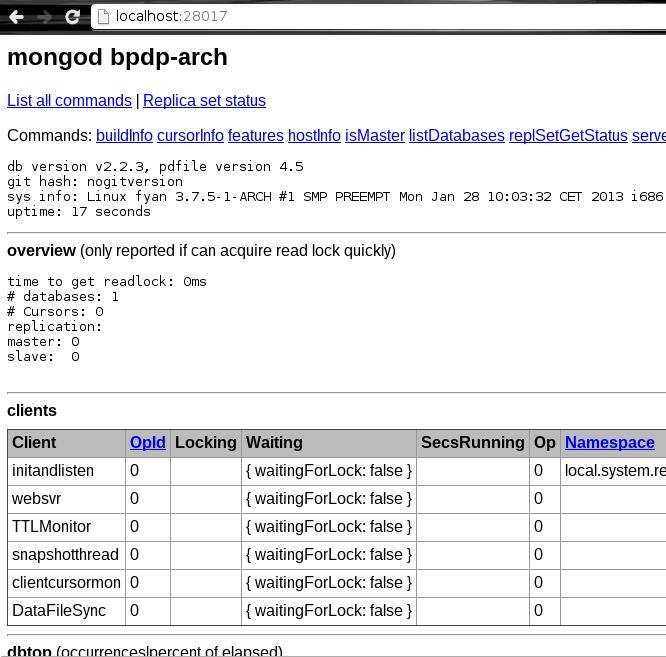
\includegraphics[scale=0.5]{images/mongodb-web-interface.jpg}
    \end{center}
    \caption{Admin web console untuk mongoDB}
    \label{fig:mongowebadminconsole}
  \end{figure}


\subsection{Documents dan Collections}

Konsep dasar yang harus dipahami dalam mongoDB sebagai \textit{document-oriented database} adalah \textit{documents} dan \textit{collections}. Sama halnya dengan basis data relasional, mongoDB menyimpan data dalam suatu basis data. Di dalam basis data tersebut terdapat \textit{collections} yang bisa diibaratkan seperti tabel dalam basis data relasional. \textit{Collections} digunakan untuk menyimpan dokumen (\textit{documents}). Dalam istilah basis data relasional, \textit{documents} adalah \textit{records}. Kerjakan latihan berikut untuk memahami pengertian dari \textit{documents} dan \textit{collections}.

\lstset{language=bash,caption=Sesi dalam shell mongoDB}
\begin{lstlisting}
$ mongo
MongoDB shell version: 2.2.2
connecting to: test
> db
test
> use mydb
switched to db mydb
> show dbs
local	(empty)
> emp1 = { name : "Zaky", address : "Griya Purwa Asri" }
{ "name" : "Zaky", "address" : "Griya Purwa Asri" }
> emp2 = { name : "Ahmad", address : "Purwomartani", email : "zakyahmadaditya@gmail.com" }
{
	"name" : "Ahmad",
	"address" : "Purwomartani",
	"email" : "zakyahmadaditya@gmail.com"
}
> emp3 = { name : "Aditya", address : "Kalasan", phone: "08787878787" }
{ "name" : "Aditya", "address" : "Kalasan", "phone" : "08787878787" }
> db.employees.insert( emp1 )
> db.employees.insert( emp2 )
> db.employees.insert( emp3 )
> show dbs
local	(empty)
mydb	0.0625GB
> db
mydb
> show collections
employees
system.indexes
> db.employees.find()
{ "_id" : ObjectId("50c74b63a7f83cba11e6b21e"), "name" : "Zaky", "address" : 
	"Griya Purwa Asri" }
{ "_id" : ObjectId("50c74b6da7f83cba11e6b21f"), "name" : "Ahmad", "address" : 
	"Purwomartani", "email" : "zakyahmadaditya@gmail.com" }
{ "_id" : ObjectId("50c74b79a7f83cba11e6b220"), "name" : "Aditya", "address" : 
	"Kalasan", "phone" : "08787878787" }
> db.employees.find( {name : "Ahmad"} )
{ "_id" : ObjectId("50c74b6da7f83cba11e6b21f"), "name" : "Ahmad", "address" : 
	"Purwomartani", "email" : "zakyahmadaditya@gmail.com" }
> db.employees.findOne()
{
	"_id" : ObjectId("50c74b63a7f83cba11e6b21e"),
	"name" : "Zaky",
	"address" : "Griya Purwa Asri"
}
> db.employees.find().limit(2)
{ "_id" : ObjectId("50c74b63a7f83cba11e6b21e"), "name" : "Zaky", "address" : 
	"Griya Purwa Asri" }
{ "_id" : ObjectId("50c74b6da7f83cba11e6b21f"), "name" : "Ahmad", "address" : 
	"Purwomartani", "email" : "zakyahmadaditya@gmail.com" }
> 
\end{lstlisting}

Basis data mongoDB hanya akan dibuat jika sudah dilakukan perintah untuk menyisipkan atau mengisikan data \textit{documents} ke dalam \textit{collections} seperti perintah di atas.

\section{Node.js dan MongoDB}

\subsection{Node-gyp}

\index{Node-gyp}Node-gyp merupakan \textit{native add-on build tool}, berfungsi untuk membantu proses kompilasi modul add-on native di Node.js. Node-gyp merupakan software bebas dan bisa diinstall menggunakan npm:

\lstset{language=bash,caption=Instalasi node-gyp}
\begin{lstlisting}
$ npm install -g node-gyp
\end{lstlisting}

Node-gyp ini diinstall pada lokasi global. Pada materi ini, Node-gyp diperlukan untuk membangun \textit{driver} dari mongoDB sehingga mongoDB bisa diakses oleh Node.js. 

\subsection{Driver Node.js untuk mongoDB}

\index{mongoDB!Driver}Mengakses mongoDB dari Node.js bisa dilakukan dengan menggunakan driver atau berbagai \textit{wrapper} serta solusi sejenis ORM \textit{Object-Relational Mapping}. Beberapa solusi yang tersedia adalah:
\lstset{language=bash,caption=Instalasi driver mongoDB}
\begin{lstlisting}
$ npm install mongodb
npm WARN package.json application-name@0.0.1 No README.md file found!
npm http GET https://registry.npmjs.org/mongodb
npm http 200 https://registry.npmjs.org/mongodb
npm http GET https://registry.npmjs.org/mongodb/-/mongodb-1.2.7.tgz
npm http 200 https://registry.npmjs.org/mongodb/-/mongodb-1.2.7.tgz
npm http GET https://registry.npmjs.org/bson/0.1.5
npm http 304 https://registry.npmjs.org/bson/0.1.5

> bson@0.1.5 install /home/bpdp/tmp/hello/node_modules/mongodb/node_modules/bson
> node install.js || (exit 0)

================================================================================
=                                                                              =
=  Attempting to build bson c++ extension                                      =
=   Windows: no build will be attempted as binaries are prepackaged            =
=   Unix: on failure the package will still install without the C++ extension  =
=                                                                              =
================================================================================
node-gyp clean
node-gyp configure build
gyp http GET http://nodejs.org/dist/v0.8.16/node-v0.8.16.tar.gz
gyp http 200 http://nodejs.org/dist/v0.8.16/node-v0.8.16.tar.gz
make[1]: Entering directory `/home/bpdp/node_modules/mongodb/node_modules/bson/build'
  CXX(target) Release/obj.target/bson/ext/bson.o
  SOLINK_MODULE(target) Release/obj.target/bson.node
  SOLINK_MODULE(target) Release/obj.target/bson.node: Finished
  COPY Release/bson.node
make[1]: Leaving directory `/home/bpdp/node_modules/mongodb/node_modules/bson/build'
child process exited with code 0
mongodb@1.2.7 ../../../../../node_modules/mongodb
+-- bson@0.1.5
\end{lstlisting}

Solusi lain yang bisa digunakan antara lain adalah:
\begin{itemize}
	\item Mongoose (\url{http://mongoosejs.com/})
	\item Mongojs (\url{https://github.com/gett/mongojs})
	\item Mongolia (\url{https://github.com/masylum/mongolia})
	\item Mongoskin (\url{https://github.com/kissjs/node-mongoskin})
\end{itemize}

\subsection{Mengakses mongoDB dari Node.js}

Dengan menggunakan \textit{collections} dan \textit{documents} di atas, kita akan mengakses data tersebut menggunakan Node.js. Untuk lebih menyederhanakan, kita akan menggunakan \textit{wrapper} dari mongoDB native driver, yaitu Mongojs. Install Mongojs lebih dahulu menggunakan npm:

\lstset{language=bash,caption=Instalasi driver mongoDB}
\begin{lstlisting}
$ npm install mongojs
npm http GET https://registry.npmjs.org/mongojs
npm http 304 https://registry.npmjs.org/mongojs
npm http GET https://registry.npmjs.org/common
npm http 304 https://registry.npmjs.org/common
mongojs@0.4.6 ../../../../../node_modules/mongojs
+-- common@0.2.1
\end{lstlisting}

Setelah itu, buat program sesuai dengan listing program berikut.

\lstset{language=bash,caption=Mengakses mongoDB dari Node.js}
\begin{lstlisting}
var databaseUrl = "localhost/mydb";
var collections = ["employees"];
var db = require("mongojs").connect(databaseUrl, collections);

// mencari pegawai bernama Aditya
db.employees.find({name: "Aditya"}, function(err, employees) {
  if( err || !employees) console.log("Tidak ada pegawai dengan nama Aditya");
  else employees.forEach( function(emps) {
    console.log(emps);
  });
});

// menyimpan data pegawai baru: Bambang
db.employees.save({name : "Bambang", address : "Yogyakarta", password: "ealhadalah", 
	sex: "male"}, function(err, saved) {
  if( err || !saved ) console.log("Pegawai 'Bambang' gagal disimpan");
  else console.log("Data pegawai 'Bambang' tersimpan");
});

// mengupdate data pegawai: Ahmad
db.employees.update({name : "Ahmad"}, {$set: {address: "Finlandia"}}, 
	function(err, updated) {
  if( err || !updated ) console.log("Data 'Ahmad' gagal diperbaharui");
  else console.log("Data 'Ahmad' berhasil diperbaharui");
});

// Hasil:
//{ _id: 50c74b79a7f83cba11e6b220,
//  name: 'Aditya',
//  address: 'Kalasan',
//  phone: '08787878787' }
//Data pegawai 'Bambang' tersimpan
//Data 'Ahmad' berhasil diperbaharui
//
// Hasil di db:
//> db.employees.find()
//{ "_id" : ObjectId("50c74b63a7f83cba11e6b21e"), "name" : 
//"Zaky", "address" : "Griya Purwa Asri" }
//{ "_id" : ObjectId("50c74b6da7f83cba11e6b21f"), "address" :
//"Finlandia", "email" : "zakyahmadaditya@gmail.com", "name" : "Ahmad" }
//{ "_id" : ObjectId("50c74b79a7f83cba11e6b220"), "name" :
//"Aditya", "address" : "Kalasan", "phone" : "08787878787" }
//{ "name" : "Bambang", "address" : "Yogyakarta", "password" : 
//"ealhadalah", "sex" : "male", "_id" : 
//ObjectId("50c75d43c111384846000001") }
//> 
//  
\end{lstlisting}

\section{Aplikasi Web Menggunakan Node.js dan mongoDB}

Contoh aplikasi web berikut hanya digunakan untuk mengambil data dari mongoDB kemudian menampilkannya di web. Data diambil dari basis data mongoDB yang sudah dibuat sebelumnya (mydb). Untuk keperluan ini, kita akan menggunakan framework Express (\url{http://expressjs.com}). Install Express di level global dengan \textit{npm install -g express}. Setelah terinstall, buat subdirektori baru (lokasi bebas) yang akan digunakan untuk menyimpan aplikasi web. Setelah itu, buat kerangka aplikasi di subdirektori tersebut sebagai berikut:

\lstset{language=bash,caption=Mengakses mongoDB dari Node.js}
\begin{lstlisting}
$ express 

   create : .
   create : ./package.json
   create : ./app.js
   create : ./public
   create : ./public/images
   create : ./public/stylesheets
   create : ./public/stylesheets/style.css
   create : ./routes
   create : ./routes/index.js
   create : ./routes/user.js
   create : ./views
   create : ./views/layout.jade
   create : ./views/index.jade
   create : ./public/javascripts

   install dependencies:
     $ cd . && npm install

   run the app:
     $ node app
\end{lstlisting}

Berikut ini adalah beberapa perubahan yang dilakukan untuk rerangka aplikasi yang dihasilkan dari perintah \textit{express} tersebut.

\lstset{language=JavaScript,caption=app.js}
\begin{lstlisting}
/**
 * Module dependencies.
 */

var express = require('express')
  , routes = require('./routes')
  , employee = require('./routes/employee')
  , http = require('http')
  , path = require('path');

var app = express();

app.configure(function(){
  app.set('port', process.env.PORT || 3000);
  app.set('views', __dirname + '/views');
  app.set('view engine', 'jade');
  app.use(express.favicon());
  app.use(express.logger('dev'));
  app.use(express.bodyParser());
  app.use(express.methodOverride());
  app.use(app.router);
  app.use(express.static(path.join(__dirname, 'public')));
});

app.configure('development', function(){
  app.use(express.errorHandler());
});

app.get('/', routes.index);
app.get('/employees', employee.list);

http.createServer(app).listen(app.get('port'), function(){
  console.log("Express server listening on port " + app.get('port'));
});
\end{lstlisting}

\lstset{language=JavaScript,caption=package.json}
\begin{lstlisting}
{
  "name": "show-employees",
  "version": "0.0.1",
  "private": true,
  "scripts": {
    "start": "node app"
  },
  "dependencies": {
    "express": "3.0.6",
    "jade": "*",
    "mongojs": "latest"
  }
}
\end{listing}

\lstset{language=JavaScript,caption=routes/index.js}
\begin{lstlisting}
/*
 * GET home page.
 */

exports.index = function(req, res){
  res.render('index', { title: 'Contoh Express+mongoDB' });
};
\end{lstlisting}

Selain itu, ada beberapa tambahan file (routes/employee.js dan views/employee.jade), penghapusan file (routes/user.js), dan perubahan yang cukup signifikan pada file \textit{views/index.jade}.

\lstset{language=JavaScript,caption=routes/employee.js}
\begin{lstlisting}
/*
 * GET employees listing.
 */

var databaseUrl = "localhost/mydb";
var collections = ["employees"];
var db = require("mongojs").connect(databaseUrl, collections);

exports.list = function(req, res){

	// mencari dan menampilkan semua pegawai
	db.employees.find(function(err, employees) {
  	res.render('employee', {listOfEmployee: employees, title: 'Daftar pegawai'});
	});

};
\end{lstlisting}

\lstset{language=html,caption=views/employee.jade}
\begin{lstlisting}
extends layout

block content
	h1= title
	p #{title}

	each employee in listOfEmployee
		p #{employee.name}
\end{lstlisting}

\lstset{language=html,caption=views/index.jade}
\begin{lstlisting}
extends layout

block content
	h1= title
	p 
		|	Selamat datang di #{title}. Aplikasi ini hanya sekedar contoh 
			aplikasi web dengan mongoDB sebagai backend. Untuk saat ini hanya 
			tersedia fasilitas untuk melihat 
		a(href="/employees") daftar pegawai.
\end{lstlisting}

 \chapter{Framework Node.js: Flatiron}

\section{Mengenal Flatiron}

\subsection{Apa itu Flatiron?}

\subsection{Fitur Flatiron}

\section{Instalasi Flatiron}

\subsection{Global}
Jika ingin menggunakan tipe instalasi ini

\subsection{Lokal}

\subsubsection{Instalasi Menggunakan npm}
\lstset{language=bash,caption=Proses instalasi Flatiron}
\begin{lstlisting}
$ npm install flatiron
npm http GET https://registry.npmjs.org/flatiron
npm http 304 https://registry.npmjs.org/flatiron
npm http GET https://registry.npmjs.org/broadway/0.2.5
npm http GET https://registry.npmjs.org/director/1.1.0
npm http GET https://registry.npmjs.org/pkginfo/0.2.3
npm http GET https://registry.npmjs.org/prompt/0.2.6
npm http GET https://registry.npmjs.org/optimist/0.3.4
npm http 304 https://registry.npmjs.org/pkginfo/0.2.3
npm http 304 https://registry.npmjs.org/prompt/0.2.6
npm http 304 https://registry.npmjs.org/director/1.1.0
npm http 304 https://registry.npmjs.org/optimist/0.3.4
npm http 304 https://registry.npmjs.org/broadway/0.2.5
npm http GET https://registry.npmjs.org/wordwrap
npm http GET https://registry.npmjs.org/read
npm http GET https://registry.npmjs.org/revalidator
npm http GET https://registry.npmjs.org/utile
npm http GET https://registry.npmjs.org/cliff/0.1.8
npm http GET https://registry.npmjs.org/eventemitter2/0.4.9
npm http GET https://registry.npmjs.org/winston
npm http GET https://registry.npmjs.org/nconf/0.6.4
npm http GET https://registry.npmjs.org/utile/0.1.2
npm http GET https://registry.npmjs.org/winston/0.6.2
npm http 304 https://registry.npmjs.org/revalidator
npm http 304 https://registry.npmjs.org/cliff/0.1.8
npm http 304 https://registry.npmjs.org/read
npm http 304 https://registry.npmjs.org/wordwrap
npm http 304 https://registry.npmjs.org/winston
npm http 304 https://registry.npmjs.org/nconf/0.6.4
npm http 304 https://registry.npmjs.org/utile/0.1.2
npm http 304 https://registry.npmjs.org/utile
npm http 304 https://registry.npmjs.org/winston/0.6.2
npm http 200 https://registry.npmjs.org/eventemitter2/0.4.9
npm http GET https://registry.npmjs.org/eventemitter2/-/eventemitter2-0.4.9.tgz
npm http GET https://registry.npmjs.org/mute-stream
npm http GET https://registry.npmjs.org/i
npm http GET https://registry.npmjs.org/async
npm http GET https://registry.npmjs.org/deep-equal
npm http GET https://registry.npmjs.org/ncp
npm http GET https://registry.npmjs.org/mkdirp
npm http GET https://registry.npmjs.org/rimraf
npm http GET https://registry.npmjs.org/colors
npm http GET https://registry.npmjs.org/cycle
npm http GET https://registry.npmjs.org/eyes
npm http GET https://registry.npmjs.org/stack-trace
npm http GET https://registry.npmjs.org/request
npm http 200 https://registry.npmjs.org/eventemitter2/-/eventemitter2-0.4.9.tgz
npm http 304 https://registry.npmjs.org/i
npm http 304 https://registry.npmjs.org/mute-stream
npm http 304 https://registry.npmjs.org/deep-equal
npm http 304 https://registry.npmjs.org/ncp
npm http 304 https://registry.npmjs.org/mkdirp
npm http 304 https://registry.npmjs.org/rimraf
npm http 304 https://registry.npmjs.org/colors
npm http 304 https://registry.npmjs.org/cycle
npm http 304 https://registry.npmjs.org/eyes
npm WARN package.json cycle@1.0.0 No README.md file found!
npm http 304 https://registry.npmjs.org/stack-trace
npm http GET https://registry.npmjs.org/deep-equal
npm http GET https://registry.npmjs.org/i
npm http GET https://registry.npmjs.org/cycle
npm http GET https://registry.npmjs.org/colors
npm http GET https://registry.npmjs.org/eyes
npm http GET https://registry.npmjs.org/mkdirp
npm http GET https://registry.npmjs.org/ncp
npm http GET https://registry.npmjs.org/rimraf
npm http GET https://registry.npmjs.org/stack-trace
npm http GET https://registry.npmjs.org/ini
npm http 304 https://registry.npmjs.org/deep-equal
npm http 304 https://registry.npmjs.org/colors
npm http 304 https://registry.npmjs.org/eyes
npm http 304 https://registry.npmjs.org/mkdirp
npm http 304 https://registry.npmjs.org/i
npm http 304 https://registry.npmjs.org/cycle
npm http 304 https://registry.npmjs.org/ncp
npm http 304 https://registry.npmjs.org/rimraf
npm http 304 https://registry.npmjs.org/stack-trace
npm http 200 https://registry.npmjs.org/async
npm http 200 https://registry.npmjs.org/ini
npm http GET https://registry.npmjs.org/ini/-/ini-1.0.5.tgz
npm http 200 https://registry.npmjs.org/ini/-/ini-1.0.5.tgz
npm http 200 https://registry.npmjs.org/request
flatiron@0.2.8 node_modules/flatiron
        pkginfo@0.2.3
        director@1.1.0
        optimist@0.3.4 (wordwrap@0.0.2)
        broadway@0.2.5 (eventemitter2@0.4.9, cliff@0.1.8, utile@0.1.2, nconf@0.6.4, winston@0.6.2)
        prompt@0.2.6 (revalidator@0.1.2, read@1.0.4, utile@0.1.5, winston@0.6.2)
$
\end{lstlisting}

Hasilnya akan terdapat pada direktori \textbf{node_modules} pada direktori aktif saat menjalankan install tersebut:

\lstset{language=bash,caption=Hasil instalasi Flatiron}
\begin{lstlisting}
$ ls -la node_modules/
total 16
drwxr-xr-x 4 bpdp users 4096 Oct  5 13:52 .
drwxr-xr-x 3 bpdp users 4096 Oct  5 13:51 ..
drwxr-xr-x 2 bpdp users 4096 Oct  5 13:52 .bin
drwxr-xr-x 8 bpdp users 4096 Oct  5 13:51 flatiron
$ ls -la node_modules/flatiron/
total 72
drwxr-xr-x 8 bpdp users  4096 Oct  5 13:51 .
drwxr-xr-x 4 bpdp users  4096 Oct  5 13:52 ..
-rw-r--r-- 1 bpdp users    26 Feb  9  2012 .npmignore
-rw-r--r-- 1 bpdp users   155 Aug 12 07:48 .travis.yml
-rw-r--r-- 1 bpdp users  1057 Feb  9  2012 LICENSE
-rw-r--r-- 1 bpdp users 12094 Aug 12 07:48 README.md
drwxr-xr-x 2 bpdp users  4096 May 23 19:02 bin
drwxr-xr-x 6 bpdp users  4096 Oct  5 13:51 examples
drwxr-xr-x 3 bpdp users  4096 Oct  5 13:51 lib
drwxr-xr-x 7 bpdp users  4096 Oct  5 13:51 node_modules
-rw-r--r-- 1 bpdp users 13732 Oct  5 13:51 package.json
drwxr-xr-x 4 bpdp users  4096 Oct  5 13:51 scaffolds
drwxr-xr-x 4 bpdp users  4096 Oct  5 13:51 test
$ 
\end{lstlisting}

\subsubsection{Konfigurasi}

Untuk menggunakan Flatiron, konfigurasi yang diperlukan hanyalah konfigurasi \textit{environment variables} dari Node.js serta Flatiron. Setelah itu, setiap kali akan menggunakan Node.js dan Flatiron, gunakan perintah \textit{source} untuk mengaktifkan. Berikut ini adalah konfigurasinya:

\lstset{language=bash,caption=Variabel lingkungan dari Flatiron}
\begin{lstlisting}
[bpdp@bpdp-arch environment]$ cat ~/environment/flatiron 
FI_HOME=/opt/master/nodejs/node_modules/flatiron

PATH=$PATH:$FI_HOME/bin

export PATH
[bpdp@bpdp-arch environment]$ 
\end{lstlisting}

Setelah itu, setiap kali akan menggunakan Node.js dan Flatiron, hanya perlu mengetikkan perintah di shell berikut ini:

\lstset{language=bash,caption=Mengaktifkan Node.js dan Flatiron}
\begin{lstlisting}
$ source ~/environment/nodejs
$ source ~/environment/flatiron
\end{lstlisting}


 \chapter{Real-time Web Menggunakan Socket.io}

\section{Apa itu Real-time Web?}

Real-time Web menunjukkan suatu pola interaksi aplikasi Web yang memungkinkan kedua sisi saling mengirimkan data saat terjadi perubahan, jadi tidak seperti pola interaksi yang menghendaki pemakai untuk me-\textit{refresh} browser jika menginginkan data / informasi / \textit{update} terbaru dari sisi server. Contoh dari real-time Web adalah Facebook dan Twitter. Pemakai akan mendapatkan \textit{update} secara langsung saat terjadi perubahan (komentar baru, pesan masuk, permintaan pertemanan, \textit{retweet}, dan lain-lain}, tanpa perlu me-\textit{refresh} halaman.

\section{Teknologi Pendukung Real-time Web}

Real-time Web merupakan hal yang relatif kompleks. Terdapat beberapa teknologi yang bisa digunakan untuk mewujudkan real-time Web tersebut. Beberapa diantaranya merupakan standar (atau akan menjadi standar), sedangkan lainnya bukan merupakan standar. 

\subsection{\textit{Ajax Technology}}

Teknologi Ajax (kadang juga ditulis AJAX, singkatan dari \textit{Asynchronous JavaScript and XML} adalah sekumpulan teknologi yang pertama kali dicetuskan oleh Jesse James Garrett. Ajax memungkinkan browser untuk mengirim data dan mengambil data dari server secara \textit{asynchronous} (di latar belakang) tanpa mengganggu keseluruhan tampilan halaman Web. Kumpulan teknologi yang digunakan adalah:
\begin{itemize}
	\item (X)HTML dan CSS untuk presentasi halaman Web
	\item DOM (\textit{Document Object Model}) untuk menampilkan data secara dinamis
	\item XML dan XSLT untuk pertukaran data (seringkali tidak menggunakan XML tetapi JSON).
	\item Obyek XMLHttpRequest untuk komunikasi asynchronous
	\item JavaScript
\end{itemize}

\subsection{Comet dan \textit{Push Technology}}

Comet merupakan istilah payung yang merangkum berbagai teknologi \textit{push}, yaitu teknologi yang memungkinkan server untuk mengirimkan data ke browser tanpa diminta oleh browser.

\subsubsection{SSE (\textit{Server-Sent Events})}

SSE merupakan bagian dari spesifikasi standar HTML5 (bisa diakses di \url{http://dev.w3.org/html5/eventsource/}. Spesifikasi ini memungkinkan server untuk mem-\textit{push} data ke halaman Web menggunakan protokol HTTP. Meski masih dalam pengembangan, tetapi beberapa browser sudah mendukung (misalnya Google Chrome / Chromium) serta Safari. Beberapa peranti pengembangan di sisi server juga sudah mendukung spesifikasi ini. Pada Node.js, pemrogram bisa menggunakan paket sse, nsse, atau EventSource.

\subsubsection{Bayeux Protocol}

Protokol ini dikembangkan oleh \textit{the Dojo Foundation} yang mengembangkan software Dojo Toolkit. Protokol ini digunakan sebagai transport untuk pesan-pesan asynchronous melalui HTTP dengan latensi yang rendah antara klien dengan server. Pesan-pesan tersebut di-rute-kan melalui channel-channel yang diberi nama dan bisa dikirimkan ke:
\begin{itemize}
	\item server ke klien
	\item klien ke server
	\item klien ke klien (melalui server)
\end{itemize}

Spesifikasi lengkap dari protokol ini bisa dilihat di \url{http://svn.cometd.com/trunk/bayeux/bayeux.html}.

\subsubsection{BOSH Protocol}

BOSH (Bidirectional-streams Over Synchronous HTTP) adalah protokol transport yang mengemulasi stream dua arah antara dua entitas (misalnya antara klien dengan server) dengan menggunakan banyak HTTP req/resp yang synchronous tanpa memerlukan polling yang sering atau respon yang terpotong-potong. Spesifikasi ini dikembangkan oleh komunitas serta yayasan XMPP dan bisa dilihat secara lengkap di \url{http://xmpp.org/extensions/xep-0124.html}

\subsection{WebSocket}

WebSocket merupakan teknologi Web yang menyediakan saluran komunikasi full duplex pada satu koneksi TCP. Protokol WebSocket distandarkan oleh IETF di RFC 6455 sedangkap API (\textit{Application Programming Interface}) dikembangkan dan distandarkan oleh W3C sebagai bagian dari HTML5. Komunikasi antara klien dengan server dilaksanakan menggunakan TCP dengan nomor port 80.

WebSocket diimplementasikan di sisi server dan klien dan memungkinkan adanya interaksi yang lebih real-time daripada teknologi push karena protokol dan API ini diimplementasikan dan bisa digunakan di sisi klien maupun server. Browser yang sudah mendukung protokol dan API WebSocket ini adalah Chrome, Firefox, Safari, Opera, dan Internet Explorer. 

Perkembangan dari WebSocket bisa dilihat dan diikuti di \url{http://www.websocket.org/}

\section{Socket.io}

\subsection{Apa itu Socket.io?}

\textit{Socket.io} adalah pustaka JavaScript yang merupakan implementasi dari protokol WebSocket serta berbagai improvisasi lain yang diperlukan untuk real-time web (\textit{heartbeats, timeouts}, dan \textit{disconnection}). Protokol transport yang didukung adalah sebagai berikut:
\begin{itemize}
\item WebSocket
\item Adobe Flash Socket
\item AJAX long polling
\item AJAX multipart streaming
\item Forever Iframe
\item JSONP Polling
\end{itemize}
Pustaka ini terdiri atas pustaka untuk sisi klien (browser) dan server (menggunakan Node.js). Browser yang didukung adalah:
\begin{itemize}
\item Internet Explorer 5.5+ (desktop)
\item Safari 3+ (desktop)
\item Google Chrome 4+ (desktop)
\item Firefox 3+ (desktop)
\item Opera 10.61+ (desktop)
\item iPhone Safari (mobile)
\item iPad Safari (mobile)
\item Android WebKit (mobile)
\item WebOs WebKit (mobile)
\end{itemize}

\subsection{Menggunakan Socket.io untuk Real-time Web}

Socket.io melibatkan sisi klien dan sisi server. Pada sisi server, paket yang diperlukan adalah cocket.io, sementara untuk sisi klien (browser), diperlukan socket.io-client. Paket socket.io-client tidak diperlukan langsung pada sisi node\_modules, tetapi ada beberapa file yang harus ditempatkan pada akses publik dengan maksud supaya bisa digunakan oleh browser. 

\subsubsection{Tentang Aplikasi}

Aplikasi ini hanya merupakan contoh kecil dari real-time Web. Aplikasi terdiri atas sisi server dan klien/browser. Pada sisi server, aplikasi ini akan mengirimkan data ke browser (push). Sementara itu, browser akan menerima hasil push tersebut dan menampilkannya kemudian mengirimkan data ke server tanpa perlu melakukan proses \textit{refresh}. Server hanya akan menampilkan data yang dikirimkan browser. 

\subsubsection{Membuat Kerangka Aplikasi dengan ExpressJS}

Untuk membuat aplikasi ini, kita akan menggunakan ExpressJS dan Socket.io. Pada awalnya, kita akan membuat kerangka aplikasi menggunakan express (jika ExpressJS belum terinstall, install dengan menggunakan \textit{npm install -g express}. 

\lstset{language=Bash,caption=Membuat kerangka aplikasi dengan ExpressJS}
\begin{lstlisting}
$ express 

   create : .
   create : ./package.json
   create : ./app.js
   create : ./public
   create : ./public/images
   create : ./public/stylesheets
   create : ./public/stylesheets/style.css
   create : ./routes
   create : ./routes/index.js
   create : ./routes/user.js
   create : ./views
   create : ./views/layout.jade
   create : ./views/index.jade
   create : ./public/javascripts

   install dependencies:
     $ cd . && npm install

   run the app:
     $ node app
\end{lstlisting}

Pada pembahasan berikutnya, kita akan mengadakan berbagai perubahan yang diperlukan.

\subsubsection{Instalasi Paket yang Diperlukan}

File \textit{package.json} berisi beberapa informasi tentang aplikasi ini serta beberapa paket yang diperlukan. Isi dari file ini adalah sebagai berikut:

\lstset{language=JavaScript,caption=package.json}
\begin{lstlisting}
{
  "name": "socket.io-expressjs",
  "version": "0.0.1",
  "author": "Bambang Purnomosidi D. P.",
  "private": true,
  "scripts": {
    "start": "node app"
  },
  "dependencies": {
    "express": "latest",
    "jade": "*",
    "socket.io": "latest",
    "socket.io-client": "latest"
  }
}
\end{lstlisting}

Setelah itu. install paket-paket tersebut dengan menggunakan perintah \textit{npm install} di direktori tersebut. 

\subsubsection{Konfigurasi JavaScript untuk Browser}

Browser juga memerlukan pustaka untuk Socket.io yang diperoleh dari paket \textit{socket.io-client}. Pada paket tersebut, terdapat direktori \textit{dist}:

\lstset{language=Bash,caption=Isi direktori dist di socket.io-client}
\begin{lstlisting}
$ ls node_modules/socket.io-client/dist/
total 496
drwxr-xr-x 2 bpdp users   4096 Dec 16 20:18 .
drwxr-xr-x 7 bpdp users   4096 Dec 16 20:18 ..
-rw-r--r-- 1 bpdp users 101222 Nov  2 22:02 socket.io.js
-rw-r--r-- 1 bpdp users  44789 Nov  2 22:02 socket.io.min.js
-rw-r--r-- 1 bpdp users 175953 Mar 28  2012 WebSocketMainInsecure.swf
-rw-r--r-- 1 bpdp users 175830 Mar 28  2012 WebSocketMain.swf
\end{lstlisting}

\textit{Copy}-kan file-file tersebut ke direktori \textit{public/javascripts}.

\subsubsection{Hapus File yang Tidak Diperlukan}

Ada beberapa file yang tidak diperlukan dan harus dihapus:
\begin{itemize}
	\item routes/user.js
\end{itemize}

\subsubsection{Ubah File-file Tertentu}

Beberapa file akan diedit. Beberapa diantaranya akan diuraikan di bagian ini.

\lstset{language=JavaScript,caption=app.js}
\begin{lstlisting}
var express = require('express')
		, app = express()
  	, routes = require('./routes')
	  , http = require('http')
		, server = http.createServer(app)
	  , io = require('socket.io').listen(server);

server.listen(80);

app.configure(function(){
  app.set('views', __dirname + '/views');
  app.set('view engine', 'jade');
  app.use(express.favicon());
  app.use(express.logger('dev'));
  app.use(express.bodyParser());
  app.use(express.methodOverride());
	app.use(express.static(__dirname + '/public'));
  app.use(app.router);
});

app.get('/', routes.index);

io.sockets.on('connection', function (socket) {
	socket.emit('kirim ke browser', { 
		kalimatDariServer: 'Kalimat ini dikirim dari server' });
	socket.on('dari browser', function (data) {
		console.log(data.kalimatDariBrowser);
	});
});
\end{lstlisting}

\lstset{language=html,caption=views/index.jade}
\begin{lstlisting}
extends layout

block content
  h1= title
  p #{title}
  script(src="/javascripts/socket.io.js")
  script
    var socket = io.connect('http://localhost');
    socket.on('kirim ke browser', function (data) {
      document.getElementById("container").innerHTML=
        "<p>" + data.kalimatDariServer + "</p>";
      socket.emit('dari browser', { 
        kalimatDariBrowser: 'Kalimat ini dikirim dari browser' });
    });
  #container
    p #{title}
\end{lstlisting}

\lstset{language=html,caption=routes/index.js}
\begin{lstlisting}
/*
 * GET home page.
 */

exports.index = function(req, res){
  res.render('index', { title: 'Contoh Socket.io + Express' });
};
\end{lstlisting}

\subsubsection{Menjalankan Server Socket.io}

Server socket.io menggunakan port 80 sehingga harus dijalankan oleh \textit{root}. 

\lstset{language=Bash,caption=Menjalankan server Socket.io}
\begin{lstlisting}
# node app.js 
   info  - socket.io started
   debug - client authorized
   info  - handshake authorized qrMUlAcSRMywnvUK31RV
   debug - setting request GET /socket.io/1/websocket/qrMUlAcSRMywnvUK31RV
   debug - set heartbeat interval for client qrMUlAcSRMywnvUK31RV
   debug - client authorized for 
   debug - websocket writing 1::
   debug - websocket writing 5:::{"name":"kirim ke browser","args":[{"kalimatDariServer":"Kalimat ini dikirim dari server"}]}
Kalimat ini dikirim dari browser
GET / 200 44ms - 628
   info  - transport end (socket end)
   debug - set close timeout for client qrMUlAcSRMywnvUK31RV
   debug - cleared close timeout for client qrMUlAcSRMywnvUK31RV
   debug - cleared heartbeat interval for client qrMUlAcSRMywnvUK31RV
   debug - discarding transport
GET /javascripts/socket.io.js 304 4ms
GET /stylesheets/style.css 304 4ms
   debug - client authorized
   info  - handshake authorized Eug556Y-X-4R8fOB31RW
   debug - setting request GET /socket.io/1/websocket/Eug556Y-X-4R8fOB31RW
   debug - set heartbeat interval for client Eug556Y-X-4R8fOB31RW
   debug - client authorized for 
   debug - websocket writing 1::
   debug - websocket writing 5:::{"name":"kirim ke browser","args":[{"kalimatDariServer":"Kalimat ini dikirim dari server"}]}
Kalimat ini dikirim dari browser
   debug - emitting heartbeat for client Eug556Y-X-4R8fOB31RW
   debug - websocket writing 2::
   debug - set heartbeat timeout for client Eug556Y-X-4R8fOB31RW
   debug - got heartbeat packet
   debug - cleared heartbeat timeout for client Eug556Y-X-4R8fOB31RW
   debug - set heartbeat interval for client Eug556Y-X-4R8fOB31RW
	 ...
	 ...
	 ...
	 ...
\end{lstlisting}

Keluaran pada sisi server tersebut merupakan keluaran yang sudah termasuk akses dari browser. Setelah server dijalankan, buka browser kemudian akses URL \url{http://localhost}. Setelah diakses melalui browser, server akan mengirimkan kode sumber HTML sebagai berikut:

\lstset{language=html,caption=Kode sumber di browser}
\begin{lstlisting}
<!DOCTYPE html>
<html>
	<head>
		<title>Contoh Socket.io + Express</title>
		<link rel="stylesheet" href="/stylesheets/style.css">
	</head>
	<body>
		<h1>Contoh Socket.io + Express</h1>
		<p>Contoh Socket.io + Express</p>
		<script src="/javascripts/socket.io.js"></script>
		<script>
			var socket = io.connect('http://localhost');
			socket.on('kirim ke browser', function (data) {
			  document.getElementById("container").innerHTML=
			    "<p>" + data.kalimatDariServer + "</p>";
			socket.emit('dari browser', { 
		    kalimatDariBrowser: 'Kalimat ini dikirim dari browser' });
			});
		</script>
		<div id="container">
			<p>Contoh Socket.io + Express</p>
		</div>
	</body>
</html>
\end{lstlisting}

Tampilan di browser bisa dilihat pada gambar~\ref{fig:socket-io-express}

  \begin{figure}
    \begin{center}
      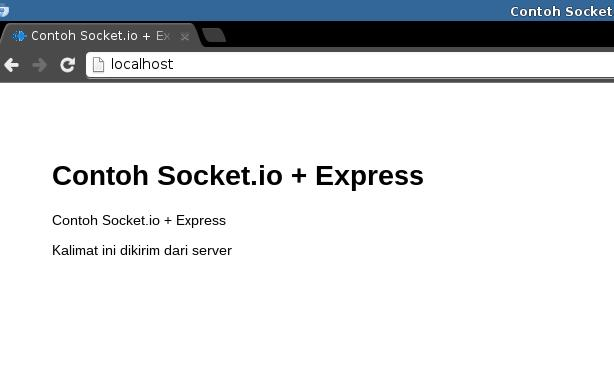
\includegraphics[scale=0.5]{images/socket-io-expressjs.jpg}
    \end{center}
    \caption{Hasil di browser dari ExpressJS + Socket.io}
    \label{fig:socket-io-express}
  \end{figure}

Contoh pada materi ini merupakan contoh sederhana, tetapi diharapkan bisa dengan mudah dipahami untuk membuat aplikasi Web real-time. 

 \begin{thebibliography}{99}
\addcontentsline{toc}{chapter}{\numberline{}Daftar Pustaka}

\bibitem{nodeuprunning}Tom Hughes-Croucher, Mike Wilson, \textit{Node: Up and Running}, O'Reilly, 2012.
\bibitem{eloquentjs}Marijn Haverbeke, \textit{Eloquent JavaScript: A Modern Introduction to Programming}, No Starch Press, 2011.
\bibitem{jsenlightenment}Cody Lindley, \textit{JavaScript Enlightenment}, \url{http://javascriptenlightenment.com}, 2012.
\bibitem{jsdefguide}David Flanagan, \textit{JavaScript: The Definitive Guide}, 4th Edition, O'Reilly, 2001.
\bibitem{jsgoodparts}Douglas Crockford, \textit{JavaScript: The Good Parts}, O'Reilly, 2008.
\bibitem{jumpstartnodejs}Don Nguyen, \textit{Jump Start Node.js}, SitePoint, 2012.
\bibitem{mdn}Anonim, \textit{Mozilla Developer Network - JavaScript}, \url{https://developer.mozilla.org/en-US/docs/JavaScript}.
\bibitem{learningnode}Shelley Powers, \textit{Learning Node}, O'Reilly, 2012.
\end{thebibliography}


 \appendix
 \appendixpage
 \addappheadtotoc

 \begin{appendices}

  \chapter{Gaya Penulisan Kode / \textit{Coding Style}}

\section{Tentang Gaya Penulisan Kode}

Pada saat seseorang berada pada proses pembuatan kode sumber (\textit{coding}), apapun gaya penulisan programnya, tidak akan bermasalah jika program itu hanya dia buat untuk si pemrogram itu sendiri. Meski demikian, hal tersebut jarang terjadi karena biasanya selalu ada kerja kelompok atau setidaknya program tersebut akan digunakan oleh pihak lain yang suatu saat perlu memahami apa yang tertulis di kode sumber tersebut. Untuk keperluan itu, biasanya diperlukan suatu gaya penulisan kode. Saat ini banyak sekali gaya penulisan kode untuk JavaScript / Node.js, biasanya tergantung pada kesepakatan anggota-anggota dalam kelompok pengembang dan berdasarkan pada pengalaman mereka tersebut. Pada lampiran ini, gaya penulisan kode dari NPM akan dituliskan secara utuh (dalam bahasa aslinya dengan harapan bisa bermanfaat untuk penyeragaman dan kemudahan membaca atau menelusuri \textit{bugs/errors}). Gaya penulisan kode ini diambil dari \url{https://npmjs.org/doc/coding-style.html}.

\section{npm's Coding Style}

npm's "funny" coding style

\subsection{DESCRIPTION}
npm's coding style is a bit unconventional. It is not different for difference's sake, but rather a carefully crafted style that is designed to reduce visual clutter and make bugs more apparent.

If you want to contribute to npm (which is very encouraged), you should make your code conform to npm's style.

\subsection{Line Length}
Keep lines shorter than 80 characters. It's better for lines to be too short than to be too long. Break up long lists, objects, and other statements onto multiple lines.

\subsection{Indentation}
Two-spaces. Tabs are better, but they look like hell in web browsers (and on github), and node uses 2 spaces, so that's that.

Configure your editor appropriately.

\subsection{Curly braces}

Curly braces belong on the same line as the thing that necessitates them. Bad:

\lstset{language=Javascript,caption=Bad curly braces placement - 1}
\begin{lstlisting}
function ()
{
\end{lstlisting}
  
Good:

\lstset{language=Javascript,caption=Good curly braces placement - 1}
\begin{lstlisting}
function () {
\end{lstlisting}

If a block needs to wrap to the next line, use a curly brace. Don't use it if it doesn't. Bad:

\lstset{language=Javascript,caption=Bad curly braces placement - 2}
\begin{lstlisting}
if (foo) { bar() }
while (foo)
  bar()
\end{lstlisting}

Good:

\lstset{language=Javascript,caption=Good curly braces placement - 2}
\begin{lstlisting}
if (foo) bar()
while (foo) {
  bar()
}
\end{lstlisting}

\subsection{Semicolons}

Don't use them except in four situations:

\begin{itemize}
  \item \textbf{for (;;) loops}. They're actually required.
  \item null loops like: \textbf{while (something) ;} (But you'd better have a good reason for doing that.)
  \item \textbf{case "foo": doSomething(); break}
  \item In front of a leading \textbf{(} or \textbf{[} at the start of the line. This prevents the expression from being interpreted as a function call or property access, respectively.
\end{itemize}

Some examples of good semicolon usage:

\lstset{language=Javascript,caption=Good semicolon usage}
\begin{lstlisting}
;(x || y).doSomething()
;[a, b, c].forEach(doSomething)
for (var i = 0; i < 10; i ++) {
  switch (state) {
    case "begin": start(); continue
    case "end": finish(); break
    default: throw new Error("unknown state")
  }
  end()
}
\end{lstlisting}

Note that starting lines with - and + also should be prefixed with a semicolon, but this is much less common.

\subsection{Comma First}

If there is a list of things separated by commas, and it wraps across multiple lines, put the comma at the start of the next line, directly below the token that starts the list. Put the final token in the list on a line by itself. For example:

\lstset{language=Javascript,caption=Comma first}
\begin{lstlisting}
var magicWords = [ "abracadabra"
                 , "gesundheit"
                 , "ventrilo"
                 ]
  , spells = { "fireball" : function () { setOnFire() }
             , "water" : function () { putOut() }
             }
  , a = 1
  , b = "abc"
  , etc
  , somethingElse
\end{lstlisting}

\subsection{Whitespace}

Put a single space in front of ( for anything other than a function call. Also use a single space wherever it makes things more readable.

Don't leave trailing whitespace at the end of lines. Don't indent empty lines. Don't use more spaces than are helpful.

\subsection{Functions}

Use named functions. They make stack traces a lot easier to read.

\subsection{Callbacks, Sync/async Style}

Use the asynchronous/non-blocking versions of things as much as possible. It might make more sense for npm to use the synchronous fs APIs, but this way, the fs and http and child process stuff all uses the same callback-passing methodology.

The callback should always be the last argument in the list. Its first argument is the Error or null.

Be very careful never to ever ever throw anything. It's worse than useless. Just send the error message back as the first argument to the callback.

\subsection{Errors}

Always create a new Error object with your message. Don't just return a string message to the callback. Stack traces are handy.

\subsection{Logging}

Logging is done using the npmlog utility.

Please clean up logs when they are no longer helpful. In particular, logging the same object over and over again is not helpful. Logs should report what's happening so that it's easier to track down where a fault occurs.

Use appropriate log levels. See config(1) and search for "loglevel".

\subsection{Case, naming, etc.}

\begin{itemize}
  \item Use \textbf{lowerCamelCase} for multiword identifiers when they refer to objects, functions, methods, members, or anything not specified in this section.
  \item Use \textbf{UpperCamelCase} for class names (things that you'd pass to "new"). 
  \item Use \textbf{all-lower-hyphen-css-case} for multiword filenames and config keys.
  \item Use named functions. They make stack traces easier to follow.
  \item Use \textbf{CAPS\_SNAKE\_CASE} for constants, things that should never change and are rarely used.
  \item Use a single uppercase letter for function names where the function would normally be anonymous, but needs to call itself recursively. It makes it clear that it's a "throwaway" function.
\end{itemize}

\subsection{null, undefined, false, 0}

\begin{itemize}
  \item Boolean variables and functions should always be either \textbf{true} or \textbf{false}. Don't set it to 0 unless it's supposed to be a number.
  \item When something is intentionally missing or removed, set it to \textbf{null}.
  \item Don't set things to \textbf{undefined}. Reserve that value to mean "not yet set to anything."
  \item Boolean objects are verboten.
\end{itemize}    

\vspace{10mm}
\hrule
\vspace{10mm}

Selain gaya penulisan kode dari NPM ini, ada beberapa lagi lainnya yang bisa dilihat, antara lain:

\begin{itemize}
  \item Spludo \url{http://spludo.com/source/coding-standards/}
  \item Google JavaScript Style Guide (\url{http://google-styleguide.googlecode.com/svn/trunk/javascriptguide.xml})
  \item Felix's Node.js Style Guide (\url{http://nodeguide.com/style.html})
\end{itemize}


%  \chapter{\textit{Commit History} dari Penulis Utama dan Kontributor}

Buku ini merupakan hasil karya bersama dari beberapa penulis. Peran masing-masing penulis bisa dilihat pada bagian ringkasan dari sejarah \textit{commit}. Penulis utama adalah saya (Bambang Purnomosidi D. P), sementara pada bab 5 ada kontribusi dari Aji Kisworo Mukti. Hasil log dari git menunjukkan peran masing-masing penulis (\textit{git shortlog}):

\lstset{language=Bash,caption=\textit{Commit history}}
\lstinputlisting{src/non-nodejs/appendix-b/commit.log}

  \addcontentsline{toc}{chapter}{Indeks}
  \printindex
 \end{appendices}

\end{document}
